%%%%%%%%%%%%%%%%%%%%%%%%%%%%%%%%%%%%%%%%%%%%%%%%%%%%%%%%%%%%%%%%%%%%%%%%%%%%%%%%
%%%%%%%%%%%%%%%%%%%%%%%%%%%%%%%%%%%%%%%%%%%%%%%%%%%%%%%%%%%%%%%%%%%%%%%%%%%%%%%%
%%                                                                            %%
%% An example for writting your thesis using LaTeX                            %%
%% Original version by Luis Costa,  changes by Perttu Puska                   %%
%% Support for Swedish added 15092014                                         %%
%%                                                                            %%
%% This example consists of the files                                         %%
%%         thesistemplate.tex (versio 2.01)                                   %%
%%         opinnaytepohja.tex (versio 2.01) (for text in Finnish)             %%
%%         aaltothesis.cls (versio 2.01)                                      %%
%%         kuva1.eps                                                          %%
%%         kuva2.eps                                                          %%
%%         kuva1.pdf                                                          %%
%%         kuva2.pdf                                                          %%
%%                                                                            %%
%%                                                                            %%
%% Typeset either with                                                        %%
%% latex:                                                                     %%
%%             $ latex opinnaytepohja                                         %%
%%             $ latex opinnaytepohja                                         %%
%%                                                                            %%
%%   Result is the file opinnayte.dvi, which                                  %%
%%   is converted to ps format as follows:                                    %%
%%                                                                            %%
%%             $ dvips opinnaytepohja -o                                      %%
%%                                                                            %%
%%   and then to pdf as follows:                                              %%
%%                                                                            %%
%%             $ ps2pdf opinnaytepohja.ps                                     %%
%%                                                                            %%
%% Or                                                                         %%
%% pdflatex:                                                                  %%
%%             $ pdflatex opinnaytepohja                                      %%
%%             $ pdflatex opinnaytepohja                                      %%
%%                                                                            %%
%%   Result is the file opinnaytepohja.pdf                                    %%
%%                                                                            %%
%% Explanatory comments in this example begin with                            %%
%% the characters %%, and changes that the user can make                      %%
%% with the character %                                                       %%
%%                                                                            %%
%%%%%%%%%%%%%%%%%%%%%%%%%%%%%%%%%%%%%%%%%%%%%%%%%%%%%%%%%%%%%%%%%%%%%%%%%%%%%%%%
%%%%%%%%%%%%%%%%%%%%%%%%%%%%%%%%%%%%%%%%%%%%%%%%%%%%%%%%%%%%%%%%%%%%%%%%%%%%%%%%

\documentclass[english,12pt,a4paper,pdftex,eng,utf8]{aaltothesis}

%% To the \documentclass above
%% specify your school: arts, biz, chem, elec, eng, sci
%% specify the character encoding scheme used by your editor: utf8, latin1

\usepackage{graphicx}

%% Use this if you write hard core mathematics, these are usually needed
\usepackage{amsfonts,amssymb,amsbsy}

\usepackage{color}

\definecolor{xkcd_blue}{RGB}{3,67,223} % https://xkcd.com/color/rgb/

%% Use this if you want to get links and nice output. Works well with pdflatex.
\usepackage{hyperref}
\hypersetup{
  pdfpagemode=UseNone,
  pdfstartview=FitH,
  colorlinks=true,
  urlcolor=xkcd_blue,
  linkcolor=black,
  citecolor=black,
  pdftitle=A Model for Selecting Software Tools for Mechatronic Systems,
  pdfauthor=Fletcher Porter,
  pdfkeywords={
    Mechatronics,Control Engineering,Software Tooling,Stewart Platform,Pneumatic actuator
  }
}

\usepackage[ddmmyyyy]{datetime}
\renewcommand{\dateseparator}{.}

\usepackage{siunitx}
\usepackage{gensymb}
\usepackage{svg}
\usepackage{lipsum}  % for placeholder text
\usepackage{subcaption}
\usepackage{bigfoot} % for \verb in \footnote
\usepackage{cprotect} % for \verb in \caption


\newcommand\ie{i.e.\ }
\newcommand\eg{e.g.}

%% All that is printed on paper starts here
\begin{document}

%% Change the school field to specify your school if the automatically
%% set name is wrong
% \university{aalto-yliopisto}
% \university{aalto University}
% \school{Sähkötekniikan korkeakoulu}
% \school{School of Electrical Engineering}

%% Only for B.Sc. thesis: Choose your degree programme.
%\degreeprogram{Electronics and electrical engineering}
%%

%% ONLY FOR M.Sc. AND LICENTIATE THESIS: Specify your department,
%% professorship and professorship code.
%%
\department{Department of Mechanical Engineering}
\professorship{Mechatronics}
%%

%% Valitse yksi näistä kolmesta
%%
%% Choose one of these:
%\univdegree{BSc}
\univdegree{MSc}
%\univdegree{Lic}

%% Your own name (should be self explanatory...)
\author{Fletcher Porter}

%% Your thesis title comes here and again before a possible abstract in
%% Finnish or Swedish . If the title is very long and latex does an
%% unsatisfactory job of breaking the lines, you will have to force a
%% linebreak with the \\ control character.
%% Do not hyphenate titles.
%%
\thesistitle{A Model for Selecting Software Tools for Mechatronic Systems}

\place{Espoo}

%% For B.Sc. thesis use the date when you present your thesis.
%%
%% Kandidaatintyön päivämäärä on sen esityspäivämäärä!
\date{\today}

%% B.Sc. or M.Sc. thesis supervisor
%% Note the "\" after the comma. This forces the following space to be
%% a normal interword space, not the space that starts a new sentence.
%% This is done because the fullstop isn't the end of the sentence that
%% should be followed by a slightly longer space but is to be followed
%% by a regular space.
%%
\supervisor{Prof.\ Jari Vepsäläinen}

%% B.Sc. or M.Sc. thesis advisors(s). You can give upto two advisors in
%% this template. Check with your supervisor how many official advisors
%% you can have.
%%
\advisor{D.Sc. (tech) Olof Colonius}

%% Aalto logo: syntax:
%% \uselogo{aaltoRed|aaltoBlue|aaltoYellow|aaltoGray|aaltoGrayScale}{?|!|''}
%%
%% Logo language is set to be the same as the document language.
%% Logon kieli on sama kuin dokumentin kieli
%%
\uselogo{aaltoRed}{''}

%% Create the coverpage
%%
\makecoverpage


%% Note that when writting your master's thesis in English, place
%% the English abstract first followed by the possible Finnish abstract

%% English abstract.
%% All the information required in the abstract (your name, thesis title, etc.)
%% is used as specified above.
%% Specify keywords
%%
%% Kaikki tiivistelmässä tarvittava tieto (nimesi, työnnimi, jne.) käytetään
%% niin kuin se on yllä määritelty.
%% Avainsanat
%%
\keywords{Mechatronics,Control Engineering,Software Tooling,Stewart Platform,Pneumatic actuator}
%% Abstract text
\begin{abstractpage}[english]
Fluid power systems can be enormously complex. The chiefest complexity is in their control components due to the deep knowledge required for effective development, the need to interface with myriad heterogeneous components, and the opacity of its operation. In the IT sector, a tech stack is a known discretization of function within a system, typically used to categorize what software tools do. This enables disparate parts of a system to be developed separately. Inspired by IT tech stacks, this paper presents a model, the mechatronic tech stack, to mitigate this complexity by siloing control system behavior into discrete functions and classifying what tools can be used to meet them. The model is demonstrated on three case studies of diverse application. The theory is promising, but there are challenges in defining the most useful abstractions and interfaces.
\end{abstractpage}

%% Force a new page so that the possible English abstract starts on a new page
%%
%% Pakotetaan uusi sivu varmuuden vuoksi, jotta
%% mahdollinen suomenkielinen ja englanninkielinen tiivistelmä
%% eivät tule vahingossakaan samalle sivulle
\newpage

%% Preface
%%
%% Esipuhe
\mysection{Preface}
%\mysection{Esipuhe}
I'd like to thank my teachers for making me wise, my family and friends for making me me, and the wind for guiding me in interesting directions. \\

\vspace{5cm}
Otaniemi, \today

\vspace{5mm}
{\hfill Fletcher Porter \hspace{1cm}}

%% Force new page after preface
%%
%% Pakotetaan varmuuden vuoksi esipuheen jälkeinen osa
%% alkamaan uudelta sivulta
\newpage


%% Table of contents.
\thesistableofcontents


%% Symbols and abbreviations
\mysection{Abbreviations}

\begin{tabular}{ll}
  IT & Information Technology \\
  HTML & Hyper Text Markup Language \\
  SQL & Structured Query Language \\
  CAN & Controller Area Network \\
  ISO & International Organization for Standardization \\
  OSI & Open Systems Interconnection \\
  HTTP & Hypertext Transfer Protocol \\
  DNS & Domain Name System \\
  FTP & File Transfer Protocol \\
  IP & Internet Protocol \\
  IO & Input/Output \\
  RAM & Random Access Memory \\
  CPU & Central Processing Unit \\
  API & Application Programming Interface \\
  I2C & Inter-Integrated Circuit \\
  USB & Universal Serial Bus \\
  PLC & Programmable Logic Controller \\
  DAQ & Data Acquisition System \\
  IEC & International Electrotechnical Commission \\
  EFPA & Extension type Flexible Pneumatic Actuator \\
  EEPROM & Electronically-Erasable Programmable Read-Only Memory \\
\end{tabular}


%% Tweaks the page numbering to meet the requirement of the thesis format:
%% Begin the pagenumbering in Arabian numerals (and leave the first page
%% of the text body empty, see \thispagestyle{empty} below).
%% Additionally, force the actual text to begin on a new page with the
%% \clearpage command.
%% \clearpage is similar to \newpage, but it also flushes the floats (figures
%% and tables).
%% There is no need to change these
%%
\cleardoublepage
\storeinipagenumber
\pagenumbering{arabic}
\setcounter{page}{1}


\section{Introduction}

%% Leave first page empty
\thispagestyle{empty}

In order to study mechatronics systems, it is necessary to design and develop physical research test beds. This is especially the case in mechatronic systems, as often they have component whose high-fidelity modeling is challenging and computationally expensive. When doing research with hardware systems, before a single research question can be asked of the hardware, researchers must assemble mechanical components, hook up power electronics, and route hoses for the hydraulic and pneumatic systems. Then the most complex of them all, the control system, must be added. Its tangle of spindly wires reaches all throughout the machine, meeting at the computer, the single most complex component of any fluid power system. The requirements placed on it are immense. In high-power systems, safety invariants must be held up perfectly lest disaster strike, and close monitoring is necessary due to the low stiffness of fluid systems compared to mechanical ones.

The tools used throughout history to create mechatronic systems have changed dramatically with developments in technology.  It will be enlightening to study it briefly.

Prior to the twentieth century, there weren't mechatronic systems as such, as the computer hadn't yet been invented, but there were controllers.  In the early eighteenth century, de Réamur created a device which regulated the temperature of a furnace which had a float on a vile of mercury that was connected through a linkage to a vent for the furnace~\cite{Bennett1996}.  When the temperature went up or down, the level of the mercury would change, causing the float to move and for the vent to open or close to encourage the furnace toward a more desired temperature.  Today we would understand this as simple proportional control, but enacted by fantastic mechanical means.

Another iconic design was the mechanical governor of the seventeenth century that regulated steam engine speeds by exploiting centrifugal forces to raise and lower masses to impede changes in engine speed.  This was another proportional controller.  It was described formally by Maxwell in 1868 where he wrote about its dynamics and stability, noting that the primary stability criterion is that all the roots of the systems dynamics must have negative real parts~\cite{Maxwell1868}.  Today we understand this as the Nyquist Criterion, but it was known 60 years before Nyquist wrote about it.

There were even proportional-derivative (PD) controllers developed in this era.  The US Navy developed the Whitehead Torpedo in 1873 which was able to regulate its depth based on a setting made by sailors before firing and then was able to dive to that depth and maintain level before hitting a target~\cite{Barber1874}.  It had a piston which was moved by hydrostatic pressures, and that piston connected to a control surface which set the torpedo's trajectory~\cite{Sears1873}.  It also had a pendulum which hung freely under gravity and a linkage connected it to another control surface on the torpedo.  Together, these made for a PD controller since the angle of the torpedo was related to the rate of change of depth.

These early controllers are incredibly fascinating designs, but their creativity was only exceeded by their complexity.  These designs coerced physical phenomena---gravity, pressure, temperature, rotation---into measurement signals that could be acted upon by a linkage-based controller.  Because the phenomena were myriad, there had to be a separate solution for every different type.  And the options for amplification were limited as well.  Mercury is not usually strong enough to open a furnace vent, so a lever will amplify the force.  But for a large furnace with a heavy door, there likely won't be a practical level.  What would ease the development of controllers would be a way to abstract phenomena into a single controllable signal.  Fortunately, the twentieth century saw the advent of exploitable electricity.

With electricity, measurement could be done by finding a way to convert a phenomenon to an electrical signal and that could be provided to a controller.  Sperry was able to electrically measure the state of the sea, wind, and a ship state to create an automatic ship steering controller~\cite{Bennett1996}.  Controllers also began to proliferate in industry where they manifested as boxes that could have measurements plugged in and a control signal would come out.  However, until Black developed feedback amplification~\cite{Black1934}, it was challenging to reliably amplify low-power control signals to a power level suitable to operate a control actuator.

One interesting case from this era of control was World War Two anti-aircraft guns.  These presented a difficult control problem.  Enemy aircraft had their position and velocity identified by radar (itself a difficult task at the time).  The controller had to anticipate where to aim the missile to intercept the target accounting for both the aircraft's and the missile's trajectories, all while tramming a heavy gun~\cite{Bennett1996}.  Initially, the measurement signal was provided by a worker shouting positions to the gun from where the radar was, but this proved too much latency for effective control.  The engineers working on the gun and those working on the radar needed to collaborate to be able to develop controller where the gun and radar would work as one automatic, closed-loop system.

In the post-war period, industrial controllers got much better thanks to the development of classical control theory in the 1930s and 40s.  However, electrical control proved to be challenging to implement.  Logic was typically implemented as huge relay circuits with dozens or hundreds of relays implementing logic~\cite{Parr1993}.  These relays were prone to failure and would cause downtime on factory lines when they needed to be replaced.  The fundamental issue was that up until this time, control programs were immutable once commissioned.  If there was a change needed, it would incur a substantial recommissioning process.  This would be solved by re-programmable controllers run on computers.

Industrial computers, or programmable logic controllers as they're called, were and are just regular computers, but the computer's package is made more robust to dust, temperature, vibrations, and other difficult environmental conditions found in industrial environments~\cite{Parr1993}.  They also have specialized programming languages that are meant to model to how control programs with relay logic were conceived.  But one major disadvantage of electronic controllers was still an issue.  The wires that ran to and from sensors and actuators made for a Cthulhu-esque tangle of wires and cables that were expensive and difficult to work on.  This was improved by the final tooling innovation discussed here, fieldbus networks.

Typically control and measurement signals consisted of $\qtyrange[range-units=single,range-phrase=..]{4}{20}{\milli\ampere}$ analog signals and $\qty{24}{\volt}$ digital signals.  This meant that every single sensor and actuator needed at least two wires, one for power and one for ground, going from it to the control box.  For large-scale controllers in factories, this was expensive and untenable to maintain~\cite{Thomesse2005}.  To solve this, practitioners developed fieldbus networks to handle their input and output.  The earliest was CAMAC which was used in the 1960s for nuclear instrumentation~\cite{Thomesse2005}.  Fieldbus networks provided benefits additional to wire cleanup.  They also enable distributing control information to many machines at once on a single network, monitoring the state of the factory floor from the design or business sections of the factory, and hierarchical control, such as described by the US National Bureau of Standards AMRF control hierarchy, where more abstract elements of an industrial plants command more concrete ones.  In particular, it describes a facility, consisting of production management and manufacturing engineering, commanding the shop, or factory floor, which in turn commands individual manufacturing cells, which then command the workstations within, and then at those workstations, operators command equipment~\cite{McLean1987}.  This all can be seen in figure~\ref{fig:amrf_control_hierarchy}.  The control tooling discussed in this thesis is concerned with the business at the Equipment and Workstation level.

\begin{figure}
  \centering
  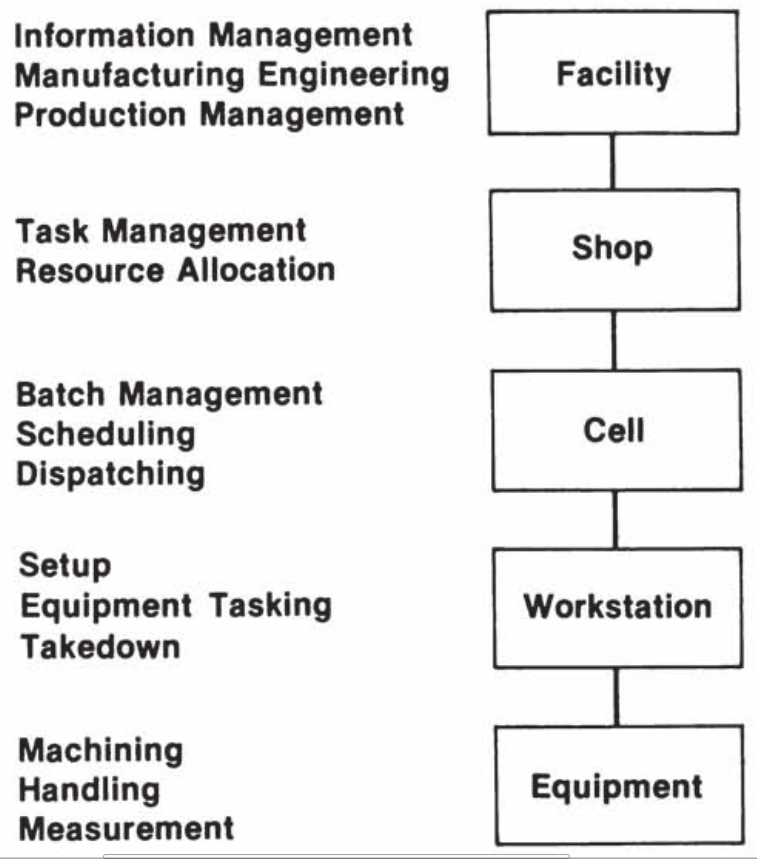
\includegraphics[width=\textwidth]{assets/amrf_control_hierarchy}
  \caption{The AMRF control hierarchy, boxed, abstracts different levels of behavior within a factory into discrete functions with well-defined interfaces between them.  Taken from~\cite{McLean1987}}\label{fig:amrf_control_hierarchy}
\end{figure}

This history has been brief, it doesn't go into the more modern tooling in robotics and its dependencies on signal libraries like ROS~\cite{ROS2}.  But what it has shown is the importance of abstraction.  Early mechanical controllers were challenging because every different physical phenomenon had to be separately and mechanically integrated into the controller.  Electricity simplified that.  Complex electrical controllers proved expensive and difficult to maintain and modify until computers moved logic to the re-programmable realm.  Finally, IO saw direct signaling abstracted to bus communication reducing massive tangles of wire to only a single cable.

This paper builds on this history to improve the process of commissioning control systems for mechatronic systems by reasoning about how to abstract the construction of behavior and components in computer control systems into layers, synthesizing a novel {\it mechatronic tech stack\/} theory, not unlike the AMRF control hierarchy. It will demonstrate in three case studies how this theory can be applied in mechatronic systems. The tools used in these cases will be categorized into layers of the mechatronic tech stack.  The analysis shows that, while different, these cases all fit into the same structure.

\clearpage


\section{Theory}

This section constructs the backbone of this paper, namely the novel theory of a mechatronic tech stack. First, there will be a review of tech stacks and {\it abstraction layers\/} as they've been applied in the IT sector. Then there will be a proposal of a mechatronic tech stack determined by a standards-based set of principles.

\subsection{Technology Stacks in the IT Sector}

The concept of a tech stack, alternately called a solution stack or a software stack, is to enumerate the tasks done by a kind of software application and to suggest tools for those tasks~\cite{PranamStack2017}. More specifically, it defines a set of abstraction layers; each layer describes a type of task and contains within it the set of software tools that complete that task. The intention is to take the difficult task of tool selection and provide a structure through which practitioners can think about the functions and tooling needs of their application, freeing mental energy to critically assess which tools would be best for their technical and personnel needs.

\subsubsection{The Web Stack}

A ubiquitous example of a tech stack in IT is the \textit{web stack}, used for developing websites and related pieces of software. The task that websites must perform, as suggested by this stack, is to present an interface to a user through a web browser (the \textit{front end}), to conduct some business logic like creating a customized page for the user (the \textit{back end}), to perform network communication (the \textit{server}), and to store and dispatch user data (the \textit{database})~\cite{PranamStack2017}. This doesn't describe all websites---many don't have databases or any real back-end logic, but it describes at least a superset of the functionality of most websites.

Tools in each of these layers are myriad and to highlight that, proceeding in figure~\ref{fig:web_stack} is a list of a small sample. Front-end tools like jQuery~\cite{jQuery} have been proven from many years of use, React~\cite{React} is very powerful and can be used in non-web contexts, and even plain HTML without an additional framework can be good on account of its simplicity. Back-end tools can allow a developer to select their favorite programming languages like Ruby or Python, or one that is specialized for web back-ends like PHP, or even JavaScript like the front end uses. Servers are often integrated into the back-end framework, but if not, specialized servers like Apache~\cite{ApacheServer} or nginx~\cite{nginx} are popular. Databases are dominated by reliable and proven relational, SQL-based offerings like MySQL or PostgreSQL, but alternatives like NoSQL or Redis~\cite{redis} have become popular in the past years.

\begin{figure}[h]
  \centering
  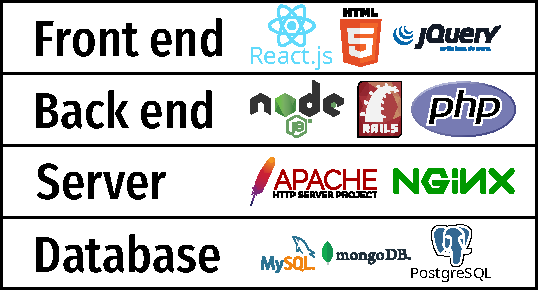
\includegraphics[width=\textwidth]{assets/web_stack}
  \caption{The web stack is like four bins of tools, here illustrated as boxes with the logos of common tools within them.}\label{fig:web_stack}
\end{figure}

In discussing the web stack, it's also useful to think about a particular set of tools used for a single project, i.e.\ one tool from each layer. Alternately, this can be thought of as the project's cross section of the web stack, or the project's own stack. There are several of these cross sections that are widely used, such as LAMP (Linux, Apache, MySQL, PHP) or MEAN (MongoDB, Express.js, Angular.js, Node.js)~\cite{PranamStack2017}. Just as often, firms employ stacks tailored to their technical and personnel needs and often write about these decisions in blog posts, such as for changes in 2023 to Microsoft Teams in~\cite{Singh2023}.

\subsubsection{OSI Network model}

Another example of a tech stack is the OSI Network model which abstractly describes network communication down to the lowest levels of physical signaling up to the highest levels of abstract behavior~\cite{ISO7498-1}. This model is frequently cited in mechatronic literature since many fieldbus protocols like CAN define their functionality in terms of this model. This model is also interesting since its standard description (ISO~7498-1) also includes principles for creating layered models of a similar ilk.

The OSI model differs from the web stack in how the layers are used by practitioners. Typically, instead of each layer being a bin to pick a tool from and where a tool must be picked from every layer which you want functionality, developers instead may decide at what depth into the model they begin their implementation and assume everything below that depth ``just works''.

The model itself consists of layered abstractions over physical communication media, as seen in figure~\ref{fig:osi_model}. The lowest OSI layer, Physical, concerns itself with the physical phenomena of communication. In the case of CAN, this means specifying voltage levels, terminating resistors, twisted pairs, grounding rules, and more. The highest level, Application, provides networking facilities without need for understanding \textit{how} the network connection is made. The Application layer includes, for example, identifying communication partners and negotiating security protocols. Well-known protocols like HTTP, SSH, and FTP exist in the Application layer. The intermediate layers provide increasing levels of abstraction over the physical layer, defining things like the structure of data packets, how to route messages, how to route them efficiently, and more.

\begin{figure}[h]
  \centering
  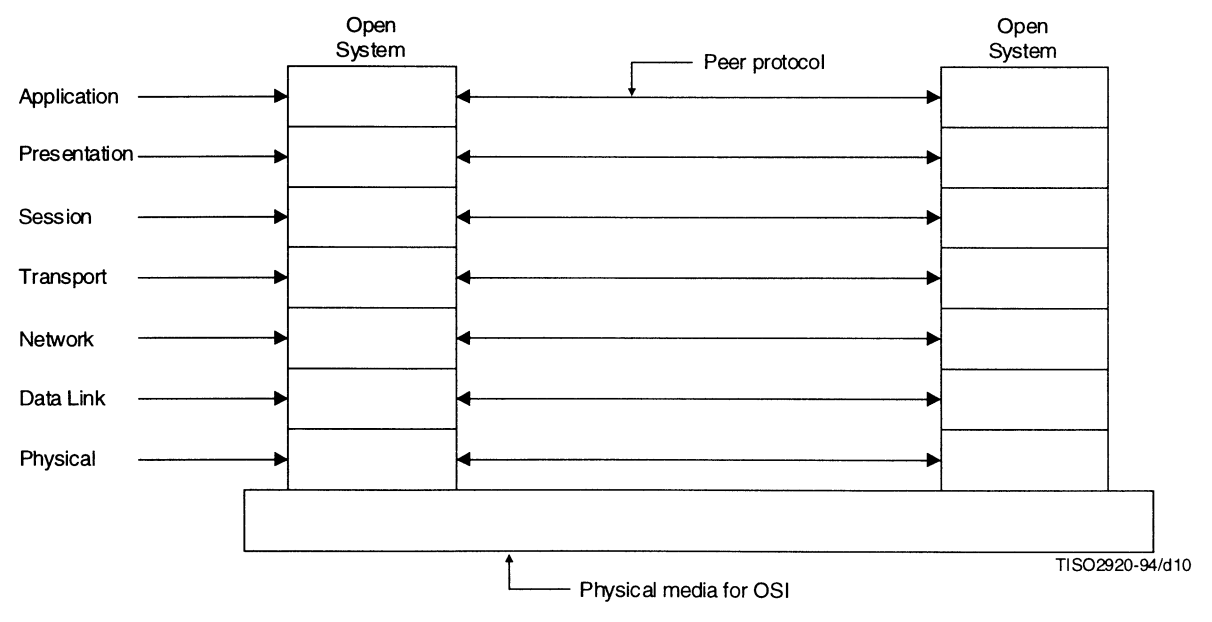
\includegraphics[width=\textwidth]{assets/osi_model}
  \caption{The OSI model understands network communication to be a layer cake of abstractions over the physical communication media.  An individual tool may implement the behaviors and interfaces of of one or multiple layers.  The layering enables design freedom in how a network is implemented.  Communication over HTTP usually goes over a TCP transport through an IP network and to other destinations over WiFi or Ethernet, but Lindgren et al.\ show that it's possible to send IP signals over CAN~\cite{Lindgren2008}, and Ethernet over EtherCAT is possible as well~\cite[§1.9.3]{EtherCATFieldbus}.  High level protocols can also be replaced to obtain a lower level of abstraction for performance or design flexibility, as was done for the video game \emph{DOOM} in 1993, as well as for contemporary game engines like Godot or Unity~\cite{DOOM1993,GodotMultiplayer,UnityTransport}.}\label{fig:osi_model}
\end{figure}

An important property of layered abstraction architectures is that protocols which are defined in higher layers can have the lower layers transparently replaced. For instance, the internet protocol (IP) which we use every day is defined in the Network layer. Typically, the internet is implemented on top of Ethernet or Wi-Fi, but with some implementation, other low-level protocols are available. Lindgren et al.\ developed IP over CAN, wherein an internet network is extended over a CAN network~\cite{Lindgren2008}, which was never imagined by the implementers of CAN nor IP.

\subsubsection{Principles for Identifying Abstraction Layers}

The OSI standard also includes the principles upon which its layers were designed~\cite[§6.2.1]{ISO7498-1}. In summary, each layer should be a discrete, separable item with a coherent function. Their interfaces should be succinct and only connect with adjacent layers. Fewer layers eases explanation and implementation and the choice of layers should be motivated by experience. This being a novel theory, experience will be the principal gain of future work, although case studies discussed later will also help. Helpfully, it offers a test to aid in determining layer boundaries. Layers should have a different level of abstraction in terms of \textit{morphology}, \textit{syntax}, and \textit{semantics}.

This model of morphology, syntax, and semantics comes from Bloomfieldian linguistics~\cite{Bloomfield1923}. It's used to coerce natural language into a structured form from which meaning can be gleaned. Here, the standard authors are using it to glean structure and meaning from engineering systems. To understand this theory, take this line of C code.

\begin{verbatim}
printf("I have %u cows\n", num_cows);
\end{verbatim}

Morphology is concerned with the atomic elements of meaning. In C code, this means short tokens of text, here \verb|printf|, \verb|(|, \verb|"I have %u cows\n"|, \verb|,|, \verb|num_cows|, \verb|)|, and \verb|;|. None of these can be reduced and still carry meaning---\verb|pri| and \verb|ntf| seperately don't combine to make \verb|printf|. But these atoms of meaning needn't be text or language. As will be discussed, they can be cables, connectors, computer hardware, or anything that carries semantic meaning.

When these tokens are combined into phrases, that's syntax. Syntax is the structure into which meaning is applied. The \verb|printf| example is syntactically parsed by C compilers as in figure~\ref{fig:printf_syntax}. The syntax tells that the postfix expression represented by the identifier \verb|printf| has the argument list of \verb|"I have %u cows\n"| (a string literal) and \verb|num_cows| (an identifier). What any of this means is the domain of semantics.

\begin{figure}[h]
  \centering
  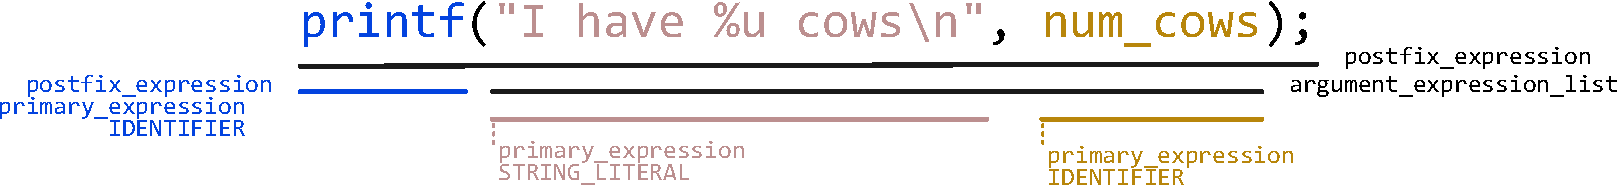
\includegraphics[width=\textwidth]{assets/printf_syntax}
  \cprotect\caption{The above printf example with syntax labeled according to Kernighan {\&} Ritchie C~\cite{Kernighan1978}.  The whole line is a postfix expression and the \verb|printf| identifier is also a postfix expression and a primary expression on its own.  The tokens between parentheses are an argument expression list, and within that, the tokens between commas are at once many types of expressions that enable writing non-trivial code, but terminating as a primary expression, and then here as a string literal and an identifier.}\label{fig:printf_syntax}
\end{figure}

The semantics of \verb|printf| are the expected behavior of the function, which can be gleaned from the documentation. It will say that \verb|printf| means to convert and write output to the console under the control of a format string~\cite{Kernighan1978}.  It will also say that the format string is the first expression in the argument expression list and that it is of type \verb|char*|.  So \verb|"I have %u cows\n"| is that format string, and the documentation will state that the second expression in the argument expression list, here \verb|num_cows| will be formatted as a string and written to the output where conversion character, here \verb|%u| is.  The logic of how the conversion characters and string formatting work are based on the format string's own morphology, syntax, and semantics, the study of which is left as an exercise to the reader.

Technology stacks, like the web stack or the OSI stack, create a structure for selecting tools for an application and abstractions for interfacing with other layers of the stack. The OSI model also provides guidance on how to architect a layered model based, among other things, on creating layers with coherent morphology, syntax, and semantics.

Next, these ideas will be used to make a mechatronic tech stack which combines the tool selecting power of the web stack and the abstract behavior of the OSI stack.

\subsection{A Mechatronic Tech Stack}

Broadly speaking, mechatronic systems include mechanical systems, power-electronic systems, and digital control systems. All of these could be considered under a theory of a mechatronic tech stack, but the present treatment will only consider the control systems. Specifically, the stack will start at the IO (input/output) interface for sensors and transducers.

The layers will be identified by noting contrasts in morphology, syntax, and semantics throughout the gamut of the control system. Layer boundaries will become evident where there are dramatic differences. I'll then describe the layers and the interfaces between them.

Morphology provides the strongest and most coarse distinctions in layers. If the atomic components of one object aren't comparable to another, they can't usefully be considered together, like comparing apples and oranges. The most obvious case is that those components that are made of literal atoms, i.e.\ hardware, must be considered separately from those that aren't physical, namely software. Within hardware, a control engineer will concern themselves with the components of the computer which their control software run on (RAM, CPU, storage, etc.) and the physical connections between the computer components and the sensors and transducers, such as cables, connectors, contacts, and traces. The software is the instructions of the control program itself, but also supporting software like the operating system, runtime environments, and libraries.

Syntax is the structure of an idea. It is a finer comb to discriminate layers. Software generally is built as a linear sequence of instructions with branches and loops. This describes the control engineer's perspective on their own control program, but supporting software like libraries are more abstract. They're better thought of as a dependency. A control program may depend on libraries A, B, and C, and those in turn depend on libraries D, E, F, and G. These \textit{middlewares}, named so as they exist in the middle between the control software and the computer, are better understood as a network of the programs themselves and the dependency connections between them. For hardware, its structure is its assemblage. The computer components are connected to the motherboard, sensors and transducers are connected to a CAN bus, the temperature sensors message over I2C, etc. Like middleware, hardware is a network of components and the connections between them, but the type of connection is also important. A system with components on a CAN bus is going to be different than one with a USB bus, and different still from a system where all components communicate over a serial connection.

Semantic meaning reveals the most subtle distinctions in layers. The control program is an expression of the business logic desired by the engineer. Middleware begins where the controller ends. It attempts to save the engineer from difficult, tedious, or uninteresting implementation otherwise necessary with computers. Computers are meaningful when they provide compelling output based on some input, i.e.\ when they compute. How this computation occurs at the hardware level is determined by the computer's \textit{architecture}. This defines what machine instructions do what and which hardware pins go where. IO is the hardware beyond the computer. It works on data transfer. A sensor's pressure reading becomes a message to the computer. The computer's actuation command becomes a message to the transducer. This is handled by e.g.\ network communication protocols, the domain of the OSI model.

This is enough to propose a mechatronic tech stack. The mechatronic stack as outlined sits on top of signaling with sensors and transducers. Those are interfaced by IO systems that connect to computer systems which run middleware upon which a control program depends. The design is so that functionality in the control layer should be preserved if components in the lower layers are changed, perhaps with some implementation effort, as was the case for IP over CAN.  This is illustrated as a stack diagram in figure~\ref{fig:mechatronic_tech_stack}.

\begin{figure}[h]
  \centering
  \includegraphics[width=\textwidth]{assets/mechatronic_tech_stack}
  \caption{The mechatronic tech stack places high-level business logic at the top and low-level interfacing at the bottom.  By siloing these function into separate layers, their behaviors and constraints can be designed separately.}\label{fig:mechatronic_tech_stack}
\end{figure}

Between the layers are the interfaces that enable higher layers to take advantage of the abstractions provided by lower layers. The control layer, being the highest, provides no interface to further layers, but from the middleware layer it demands certain \textit{application programming interfaces}, or APIs. Each program in the middleware layer generally provides an API, so the control-middleware interface is the union of all these APIs. The needs of middleware are typically met by other middleware, but those that interface with the computer directly do so through architecture-defined machine code. Then for the Computer-IO interface, the IO needs hardware connections like pins broken out from the CPU or connection ports like for CAN, serial, or Ethernet. Finally, IO interfaces with sensors and transducers in the same way it does with computers, through hardware interfaces like terminal blocks or hookups to a fieldbus.

This model, like the web stack, provides a structure through which to think about tool selection. The choice of using CAN- or serial-based IO can be understood separately from the decision of what programming language to use for the controller. This isn't to say that tooling decision in the high layers is completely decoupled from those in the low layers. The decision to use an AVR-based Arduino computer likely precludes writing the controller in JavaScript, but this is due to a lack of middleware to support that use case.

Following will be three case studies providing concrete illustrations of how this mechatronic tech stack model can be applied. These will mostly be descriptive case studies that apply this theory for retrospective research, but one case uses this model prescriptively.

\clearpage


\section{Case Studies}\label{sec:case_studies}

These case studies will apply the theory of a mechatronic tech stack to four projects---one where a requirement change caused a re-architecture of the control system, another where three similar devices have their stacks compared, the third has its stack designed with this theory in mind, and the last considers the design of a control system against challenging requirements. In all cases, the project's stack will be explicated and there will be a discussion of interesting features of its stack.

\subsection{Matlab or a PLC for a Steering Linkage?}

Dolores is a full-scale test bed in the Aalto University Fluid Power Laboratory, seen in figure~\ref{fig:dolores0} to study the application of electric hydrostatic actuation in an articulated-steering linkage for a front-loading mining vehicle~\cite{Hermansson2021, Helduser1999, Dudzinski1989}. Its control system commissioning was completed in 2021, but in 2023, an industry partner in the experiment requested hardware changes that demanded a substantial re-architecture of the control system. This case study will discuss the mechatronic tech stacks behind the old and the new systems.

\begin{figure}[h!]
  \centering
  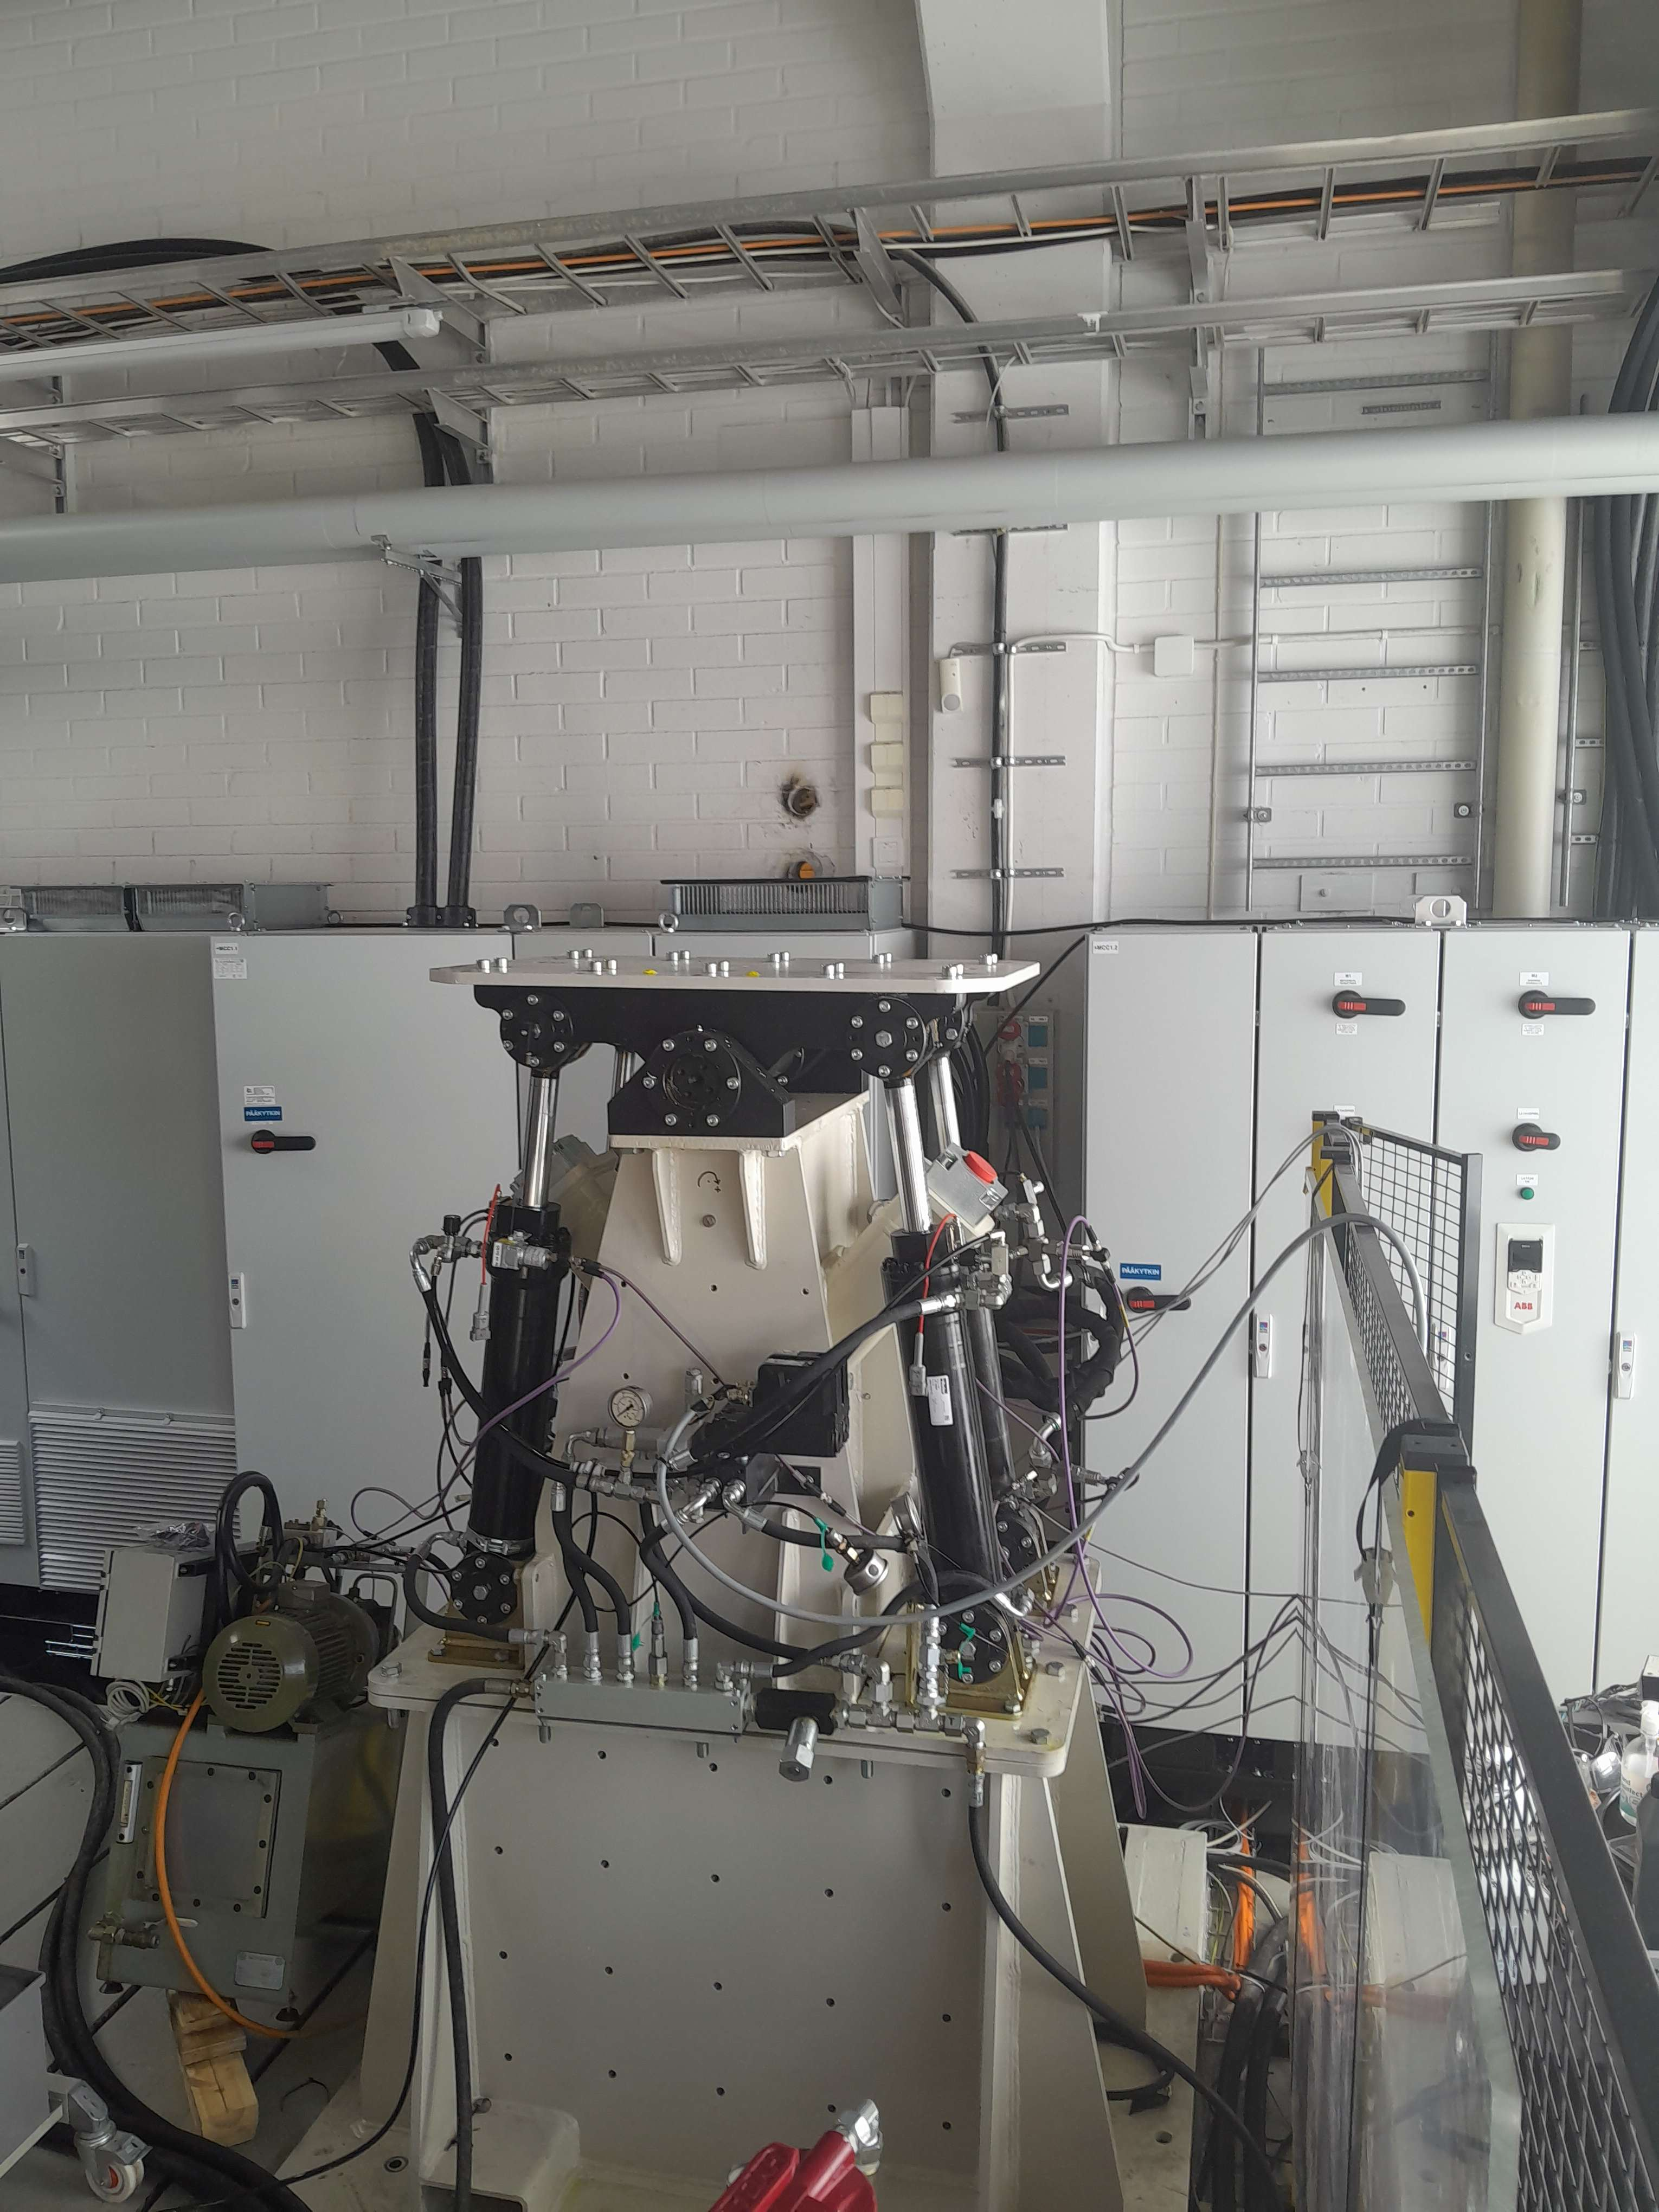
\includegraphics[width=0.8\textwidth]{assets/dolores}
  \caption{Dolores rotates the top platform about a pivot by actuating a pair of hydraulic cylinders.  A pair of additional cylinders in parallel can resist the motion providing loads useful for testing.}\label{fig:dolores0}
\end{figure}

The industry partner's requested change occurred in the IO (input/output) layer. The system has an inverter that drives a servomotor, a safety valve to enable the system, and an array of pressure, temperature, and flow sensors to observe the state of the hydraulic system. In the originally commissioned system, the inverter and the pressure and temperature sensors all communicated over a CANopen bus, the flow sensors gave analog inputs, and the safety valve was actuated with a digital signal. The CAN communication was executed by a Vector CAN/USB dongle~\cite{VectorCanUsbDongle}. All other IO went through a National Instruments data acquisition device (DAQ). In the new system, the forced change was for the inverter to communicate over EtherCAT instead of over CANopen.  The existing instrumentation didn't support EtherCAT, so this meant new IO hardware was needed to support this protocol, which was selected to be Beckhoff EtherCAT terminals. They provided the interface to connect the inverter, digital and analog IO, and a CAN bus for the sensor network~\cite{BeckhoffEL6751}. This made the DAQ unnecessary, but the CAN/USB dongle was still required due to deficiencies in Beckhoff's control interfaces that were discovered during development, which are discussed with the control layer.

The system had been controlled by a conventional Windows workstation. This may have been fine to keep for the new system, but there was concern with using a whole workstation only for a single experiment. Instead, one of Beckhoff's industrial PCs was selected as the computer to match the IO terminals and so leverage Beckhoff's support~\cite{BeckhoffC60XX}. It was expensive, but it was thought that architecting the system to align with vendor expectations would make development easier and mitigate potential problems. However, the desktop workstation did tap into the CAN bus to initialize the sensors, so it wasn't completely out of the loop.

In the old system, the workstation ran Windows, the DAQ was managed by drivers from National Instruments, and the CAN bus was initialized using Vector's CANalyzer application and runtime commands came through Vector's Simulink library~\cite{VectorCanalyzer, SimulinkVectorCAN}. Due to issues getting reliable EtherCAT connections with Simulink (possibly for user error, though the documentation wasn't clear), the new system uses a PLC-based middleware. Still based on Windows, it has libraries and runtimes to run the EtherCAT bus, to read from the CAN bus, and to interface with an external development workstation. CANalyzer remained to initialize the CAN bus.

The old system had controllers written with Matlab and Simulink. However, due to middleware issues, they were abandoned in favor of writing controllers in PLC languages based on IEC~61131-3 with the TwinCAT development environment~\cite{IEC61131-3, BeckhoffTwinCAT}. The major issue with TwinCAT is that its CANopen implementation has no documented way to initialize devices on startup. This was worked around by initializing devices with CANalyzer on the workstation.

Together, the stack for the old system was CANopen-based IO with a DAQ supplementing simple analog and digital signals, a workstation computer, Windows middleware with drivers and libraries to support communication with the CAN bus and DAQ, and a controller based on Matlab and Simulink. In the new system, the stack was a mix of EtherCAT and CANopen IO, a Beckhoff Industrial PC in concert with a workstation, PLC middleware with an application to initialize the CAN network, and a controller written in PLC languages with TwinCAT.\ This is illustrated in figure~\ref{fig:mechatronic_tech_stack_dolores}.

\begin{figure}[t]
  \centering
  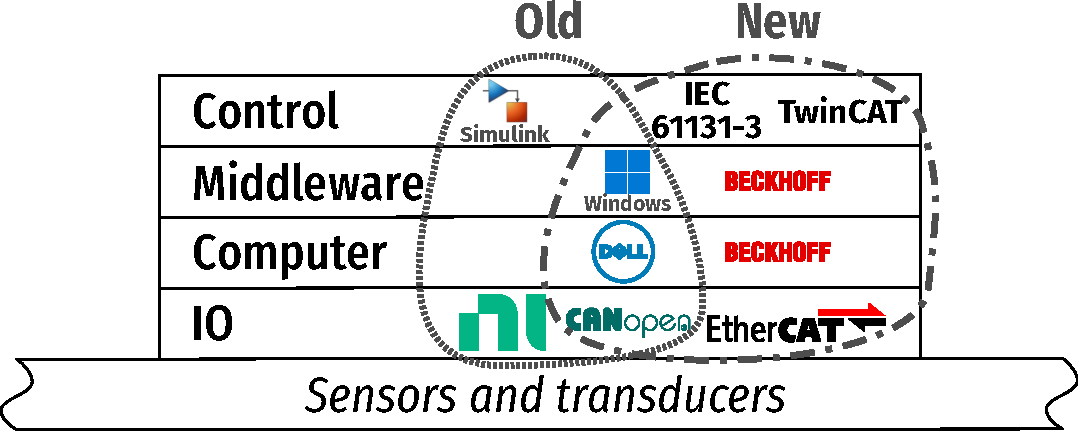
\includegraphics[width=\textwidth]{assets/mechatronic_tech_stack_dolores}
  \caption{The change was to use Beckhoff's stack, though it didn't work without supplements.}\label{fig:mechatronic_tech_stack_dolores}
\end{figure}

Notably, a small change in the system, a change in IO protocol, demanded a wholesale re-architecture of the control system. Also notable is that the CAN issues in controller-layer tooling echoed through the whole stack. This speaks to how in both stacks, the tools are \textit{tightly coupled}, meaning changes in one tool often demand changes in the others. For this mechatronic stack model to be a useful means of selecting tools like the web stack, the layers need to be \textit{loosely} coupled so tools can be replaced with minimal change in other layers.

\subsection{Embedded Systems for Soft, Pneumatic Actuators}

A research group at Okayama University of Science has, over the past years, developed a novel soft, pneumatic actuator that extends when supplied with pressure called an extension-type flexible pneumatic actuator (EFPA)~\cite{Noritsugu2005}. This section will study the tech stacks for three applications of this actuator, a six-legged mobile robot for providing the elderly with an interactive physical activity~\cite{Hase2020}, a pipe-traversal robot for inspecting and repairing water pipe networks~\cite{Shinohara2020}, and a lightweight servo valve based on bending hoses to support EFPA applications~\cite{Kobayashi2020}. All of these can be seen in figure~\ref{fig:soft_pneumatic_actuators_demo}. Note that because this is a case study on work I did not participate in, some details are not documented and must be inferred.

\begin{figure}[h]
  \centering
  \begin{subfigure}[t]{0.47\textwidth}
    \centering
    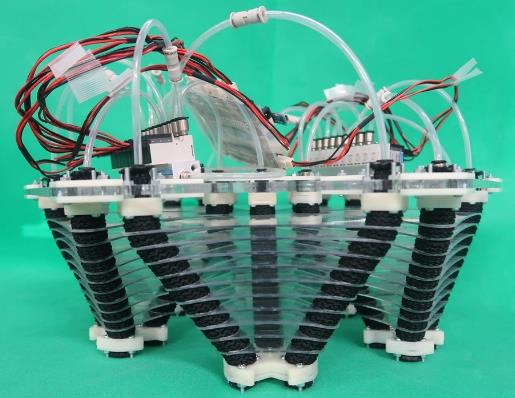
\includegraphics[width=\textwidth]{assets/six_legged_robot}
    \caption{Six-legged robot~\cite{Hase2020}}\label{sfig:six_legged_robot}
  \end{subfigure}
  \begin{subfigure}[t]{0.51\textwidth}
    \centering
    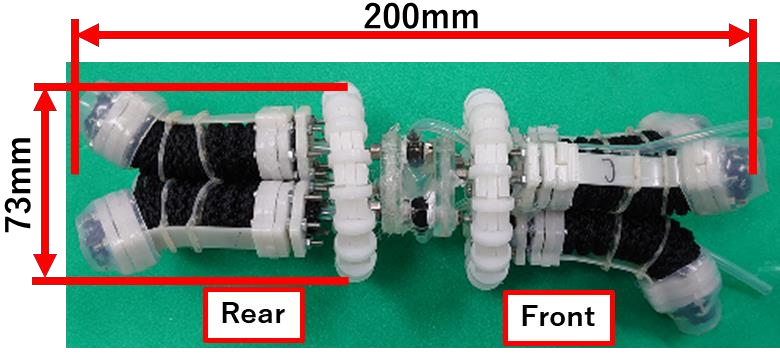
\includegraphics[width=\textwidth]{assets/pipe_robot}
    \caption{Pipe-traversal robot~\cite{Shinohara2020}}\label{sfig:pipe_robot}
  \end{subfigure}
  \begin{subfigure}[t]{0.5\textwidth}
    \centering
    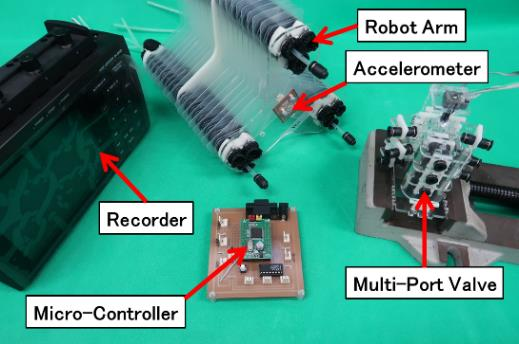
\includegraphics[width=\textwidth]{assets/bending_servo_valve}
    \caption{Bending servo valve~\cite{Kobayashi2020}}\label{sfig:bending_servo_valve}
  \end{subfigure}
  \caption{These projects are made by the same people with the same technologies using similar tools.  Photos taken from the cited papers.}\label{fig:soft_pneumatic_actuators_demo}
\end{figure}

In the IO layer, all three are similar. The six-legged and pipe robots have an array of on/off valves commanded by digital signals to pressurize their EFPAs. The servo valve has its position set with a small motor, which is controlled by a PWM signal. These signals are propagated through direct connection to pins on the computer, although Shinohara et al.\ note that there are circuits between stepping up power~\cite{Shinohara2020}. The robots received command signals from a workstation over a serial connection. Hase et al.\ note that there was an intermediate chip on the six-legged robot to connect over USB~\cite{Hase2020}. The servo valve computer had no reported inputs, though several sensors were connected to a data recording device.

The computer used for the two robots was an SH7125, a 32-bit SuperH-based system on a chip, a device that has all necessary components for computation like CPU, RAM, and peripherals on a single die~\cite{SH7125}. The servo valve used an H8/3264, a 32-bit H8/300-based system on a chip~\cite{H83264}. These architectures, while unfamiliar in name, are common for applications like printer or hard drive controllers where cost and hardware IO are important. Both CPUs have inbuilt peripherals for IO where when the CPU writes a number to a register, the IO pins will change state to match the IO register's binary representation.

No middleware is mentioned in these papers. While it's in principle possible that they ran some embedded operating system, it's doubtful given all their controllers are quite simple, as discussed below. It is possible that they used some external libraries to aid in programming.  In industry parlance, this kind of system without an operating system is a \textit{bare metal} system; so-called because that's all there is to the middleware interface.

The language the controllers were written in was not mentioned in the papers, but it's likely they used an assembly language or C since major compilers support both of these architectures~\cite{GccSupportedArchitectures}. Hase et al.\ state that the control program they wrote was to cycle through a fixed sequence of states for the valves, perhaps switching sequences interactively over the serial connection~\cite{Hase2020}.  This would be a controller based on a finite-state machine.

Each of these three projects implemented a largely similar stack---IO based on direct connections to the CPU with supporting circuitry, an embedded system-on-a-chip computer, bare metal middleware, and controllers written in C or assembly. By using a common stack, these researchers were able to skip over the tedious and difficult work of selecting tools and just use what is familiar to their institution and focus their energy on research.

\subsection{A Novel Stack for a Pneumatic Stewart Platform}\label{sec:stewart_platform}

In claiming that this mechatronic tech stack aids development, it would be prudent to start a project to study what tools this model lends itself to when applied prescriptively. The project was a driving simulator chair that had been an unfinished student project a year prior~\cite{Bjoerklund2023}. The mechanical systems had been finished including all the sensors and transducers, so all that was needed was a control system.

\begin{figure}[h]
  \centering
  \begin{subfigure}[t]{0.43\textwidth}
    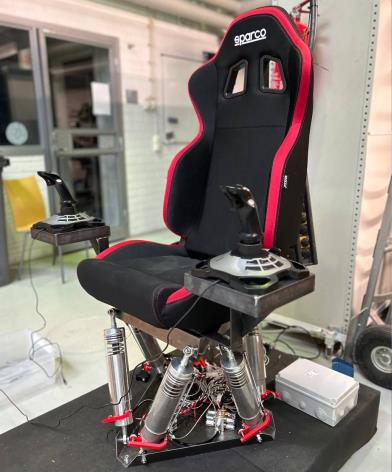
\includegraphics[width=\textwidth]{assets/rocking_chair}
  \end{subfigure}
  \quad
  \begin{subfigure}[t]{0.53\textwidth}
    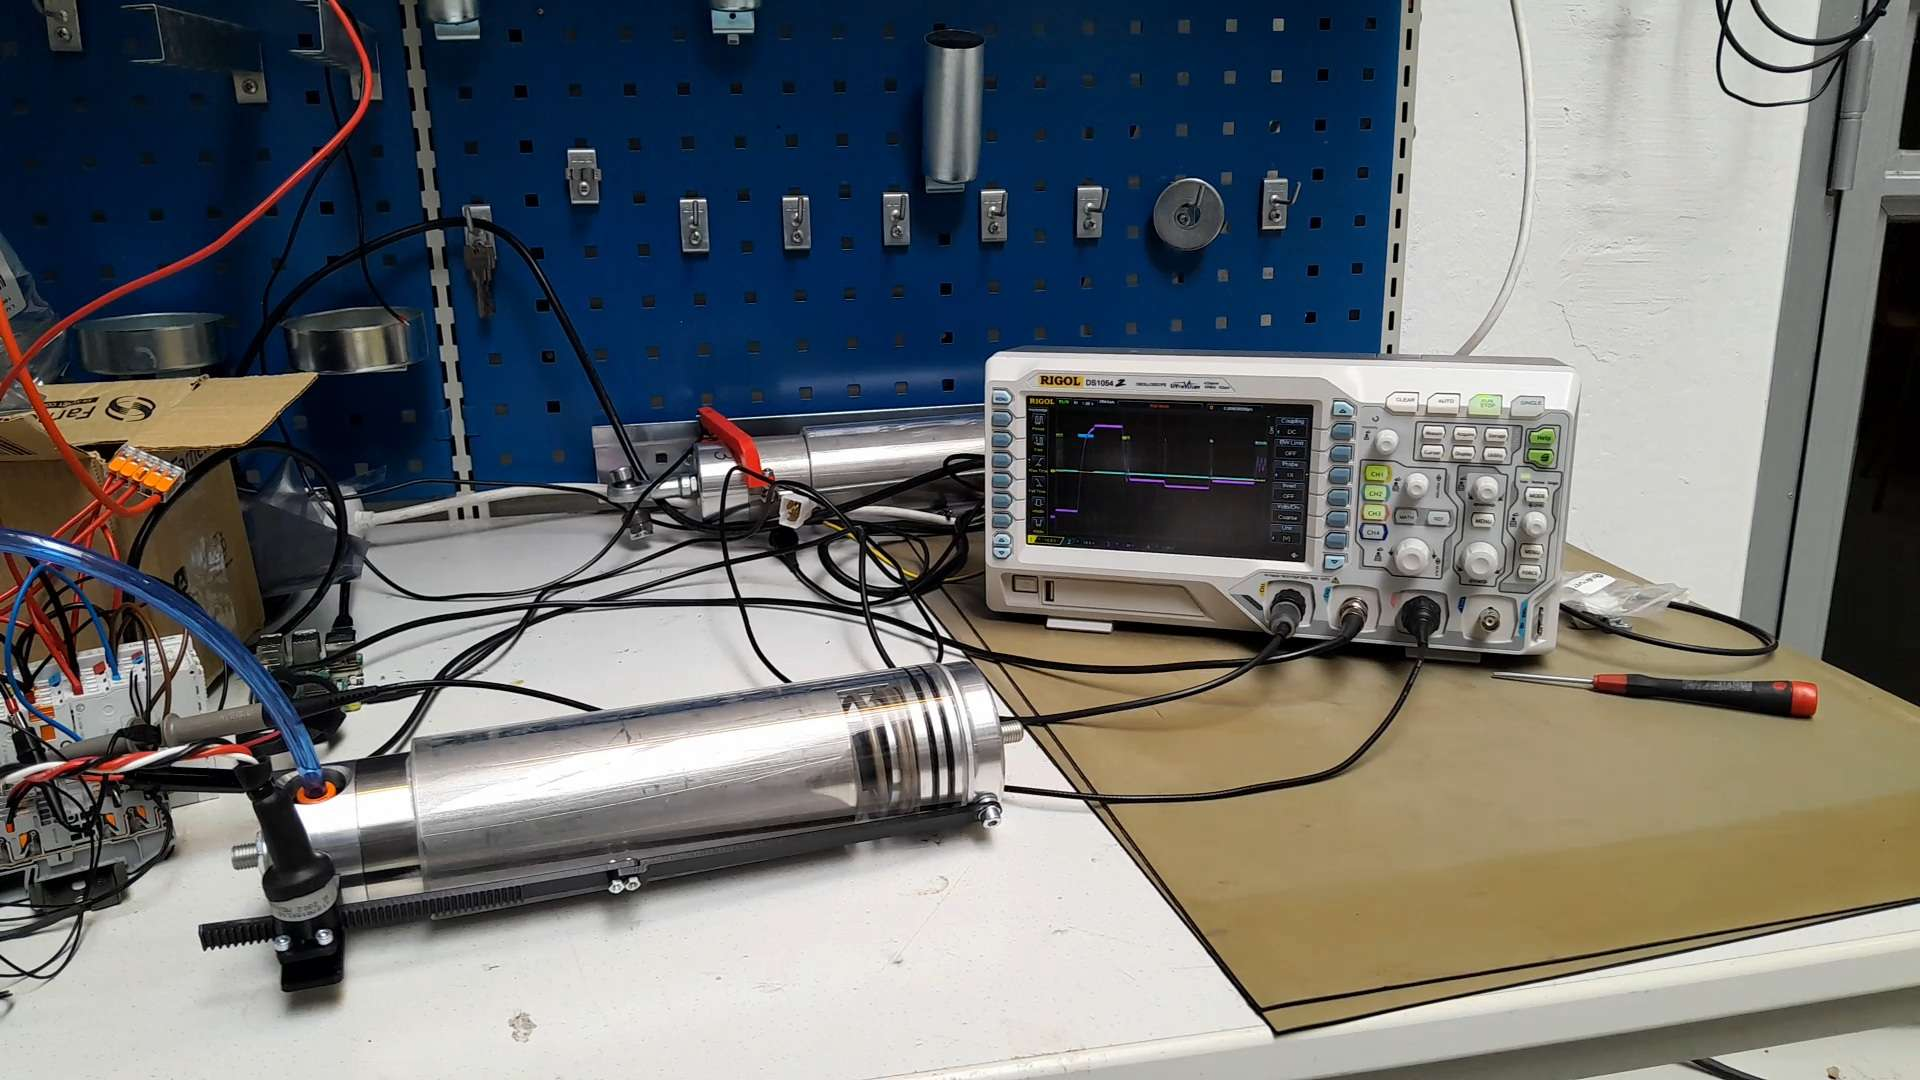
\includegraphics[width=\textwidth]{assets/pneumatic_cylinder_test}
  \end{subfigure}
  \caption{The whole system, left~\cite{Bjoerklund2023}, is a chair on a Stewart platform made with pneumatic cylinders.  On the right is a cylinder driven under the present tech stack.}\label{fig:stewart_platform_demo}
\end{figure}

The system is a chair atop a Stewart platform whose linear actuators are single-acting pneumatic-muscle cylinders, seen in figure~\ref{fig:stewart_platform_demo}~\cite{Stewart1965, Caldwell1995}. The valve manifolds that were already made for this had one valve to connect the pneumatic muscle to an external pressure source and another to vent the muscle to atmosphere. When both valves are closed, the cylinder brakes. There are six instances of this circuit, connected in series to a common pressure source. Each cylinder also has a position sensor exposed as a voltage signal from a potentiometer.

Tool selection started from the IO layer. The need was to switch 12 digital $\qty{24}{\volt}$ outputs for the valves and six analog inputs ($\qtyrange[range-units=single,range-phrase=..]{0}{24}{\volt}$) from the position sensors. It was also desirable for the work to be done quickly to have a demonstration in time for publication. This was met with EtherCAT IO cards from Beckhoff~GmbH, in large part thanks to their availability within the Aalto University Fluid Power Laboratory. They supply IO cards that mostly met the requirements; the digital outputs needed to be supplemented with flyback diodes to handle the inductive load and the analog input signals needed to be stepped down to $\qtyrange[range-units=single,range-phrase=..]{0}{10}{\volt}$ with resistors~\cite{BeckhoffEL2042,BeckhoffEL3062}. This meant routing signal cables from the sensors and transducers to terminal blocks, placing circuitry in the terminals, and then routing to the Beckhoff terminals, where there is an EtherCAT connection to the computer's Ethernet port~\cite{BeckhoffEK1100}.

In selecting the computer, it needed to communicate with the IO over EtherCAT and be cheap and easy to develop for. The Raspberry Pi supports EtherCAT, is reasonably priced, and Linux-based systems are familiar and easy to develop software for.  The simplicity of the controller that was implemented also didn't demand much from the computer.

The principal middleware requirement was an EtherCAT master, which itself depends on system-level networking. Linux satisfies the system-level networking requirement. EtherCAT masters are conventionally provided by PLC-based systems, like those from Beckhoff~\cite{BeckhoffTwinCAT}. However, they generally do not run on Linux. Additionally, their behavior is opaque and does not lend itself to understanding the system. So, Ethercrab, a master written in the Rust programming language, was used~\cite{Ethercrab}. Ethercrab benefits from being open source, so motivated users can troubleshoot more easily. It also has thorough documentation and lots of examples (e.g.\ the control-layer application was based on \verb|ethercrab/examples/ek1100.rs|). Interfacing with Rust is a benefit due to its ease of use, quality tooling, performance, and memory safety~\cite{RustHomePage}.

Finally, the control layer had to use the API of the middleware layer to implement the business logic. One case of that logic was to have a controller to regulate the position of each cylinder. It had to be implemented in Rust to interface with the Ethercrab library. It also required some code to initialize the EtherCAT communication and to configure the Beckhoff terminals. There's also a user interface to interactively set the cylinder position. An interesting issue came up where the position sensor signal, mapping the $\qtyrange[range-units=single,range-phrase=..]{0}{10}{\volt}$ IO signal to the range 0..1~\verb|float|, but only reached the range 0..0.5~\verb|float|. This was because the step-down resistor was larger than designed since the right size wasn't available, so the maximum sensor reading was smaller than $\qty{10}{\volt}$. This unhandled gain is an undesired interface between the Control and IO layers since it demands the controller be written with knowledge of the minutia of how the IO was implemented. Further research will go toward how to accommodate this.

Also interesting in the architecture of a control system is what development environments can be constructed for it.  The development environment is distinct from the so far discussed mechatronic stack since it is not a part of the function of the running system, but instead is the means which an engineer uses to turn an idea into assets for a mechatronic system.  For a given tech stack, any development environment generally can yield the same assets, but a good tech stack may lend itself to higher quality, more consistent output, faster development cycles, or at least to be more enjoyable for individual engineers to use.

For the control layer, I wrote the code in the Sublime Text text editor~\cite{SublimeText} and configured it to automatically format the source code according to standards for the Rust language using the \verb|rustfmt| utility~\cite{rustfmt}.  Other text editors like Emacs, Vim, or VSCodium would have also been good choices, but Sublime is familiar.  This was done on a Windows workstation, but it was compiled and run on the Raspberry Pi Linux control computer.  To achieve this, I checked the changes on the workstation into a \verb|git| version control repository and pushed them to the control computer\footnote{A small issue that comes up is that \verb|git| generally doesn't allow users to push changes to a branch of a repository that the local user has checked out, which is the case here~\cite[§receive.denyCurrentBranch]{GitConfig}.  This is to prevent data loss.  To enable this, \verb|git| can be configured to update the local branch only if there is no possibility of data loss by executing \verb|git config receive.denyCurrentBranch updateInstead|.}.  Then, though a remote terminal, I executed commands to compile and run the program.  This became quite annoying with how many steps there are, so I use the utility \verb|cargo-watch| to automatically execute the compile and run commands on the control computer when there are changes\footnote{The command was similar to \verb|cargo watch -x 'run -- eth0'|, which compiles and executes the program with the argument \verb|eth0|, which is the network interface the EtherCAT connection is on.}~\cite{CargoWatch}.  This still is somewhat tedious and so requires more development.  It also would have been mitigated by developing in some kind of Linux environment or by using a containerized environment like would be provided by Docker or Vagrant, which would have allowed running some tests on the development machine~\cite{DockerDev,VagrantDev}.  Most of the middleware was prepared with the Raspberry Pi OS image that was installed while commissioning the control computer, but there was some additional configuration, e.g.\ to install \verb|git|, that was done with the OS's \verb|apt| package management utility~\cite{apt}.  As well, library dependencies for the control program like Ethercrab were managed with the Rust \verb|cargo| utility~\cite{Cargo}.  The computer, once commissioned, did not require any development.  The IO layer's development was aided by a four-channel oscilloscope and a multimeter, seen in figure~\ref{fig:stewart_platform_demo}, to validate electrical connections and ensure signal were propagating as expected.  It was also interesting to observe the timing jitter of the program, which was generally very small, on the order of microseconds.

The in-depth consideration of the development environment was possible because of the open nature of all the tools considered.  Every tool, both a part of the control system and the development environment, have interfaces that enable and encourage users to compose or develop tools to make an environment that meets their needs.  This same discussion could not be had with regards to Dolores since its PLC-based system doesn't have interfaces for customization or external development, and any interfaces there are demand mastery of low-level communication protocols.  The development environment was simply whatever Beckhoff blessed; no more, no less.

This Stewart platform employed a tech stack consisting of Beckhoff EtherCAT terminals with supplementing circuits for IO, a Raspberry Pi computer, Linux and Ethercrab for middleware, and control layer built with the Rust programming language.  By crafting a custom stack with largely open components, it was easy to also consider and iterate on the development process.  This all proved to be quite successful, as all the development, including ideating on the tech stack itself and learning how to use Ethercrab, was completed in only a week and a half.

\subsection{Stress Testing IO Requirements}

The Solid Mechanics Laboratory at Aalto University conducts experiments to identify the properties of engineering materials under load particularly studying phenomena ranging from the micron to the meter scale.  As is typical for laboratories studying solid mechanics, they do this by subjecting test samples to a load schedule using a servo-controlled hydraulic cylinder as seen in figure~\ref{fig:solid_mechanics_test_rig}.  They have several test beds, each with an instance of a common control system.  This had been controlled by a workstation-commanded DAQ that communicated with a motor controller and a strain gauge amplifier, but new experiments and the desire for faster, better research cycles called for improvements to the control system.  The following discussion is based heavily on an interview I took with the lab's head Dr.~Pauli Lehto.

\begin{figure}[h]
  \centering
  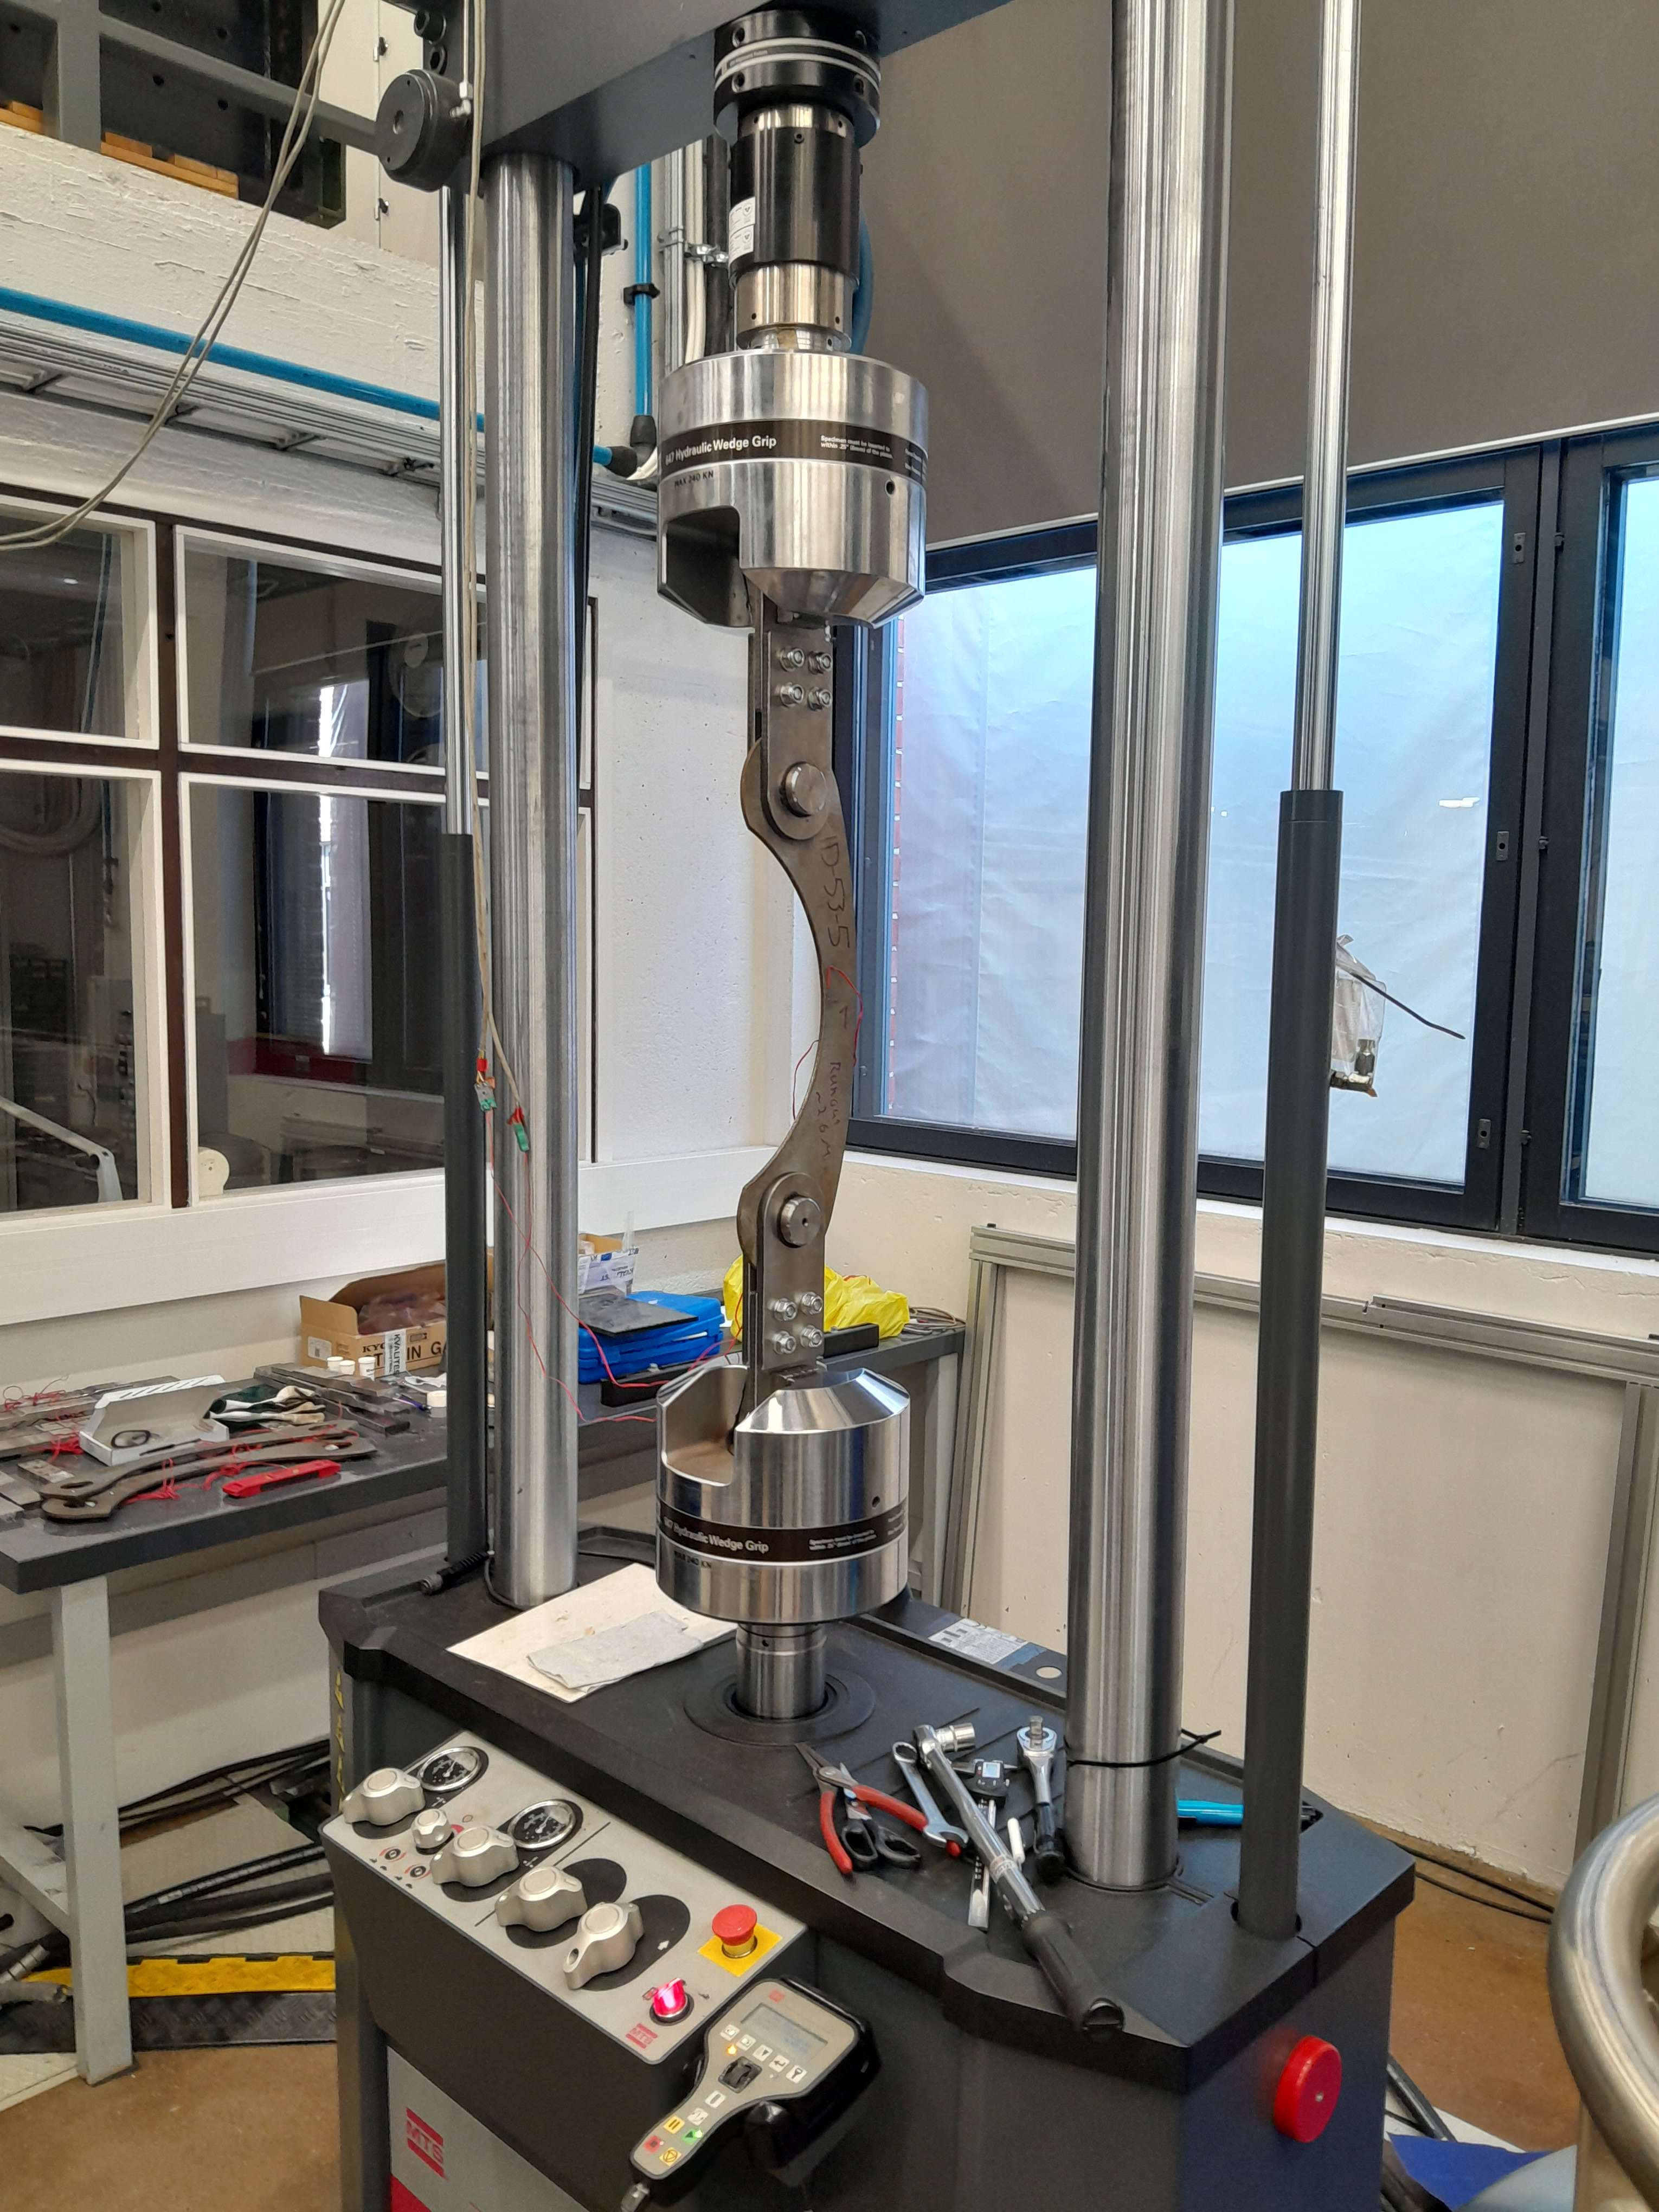
\includegraphics[width=0.90\textwidth]{assets/solid_mechanics_test_rig}
  \caption{A typical test in the solid mechanics lab, this has a sample will experience axial loads provided by the surrounding machine and sensors on and around the sample collect measurements for data acquisition and control feedback.}\label{fig:solid_mechanics_test_rig}
\end{figure}

The requirements that drive the design of this control system are mainly related to timing.  There are three compelling design parameters when it comes to timing.  The first is frequency or PID speed; how often in time do control and measurement samples occur?  According to Nyquist, the higher the frequency, the better the control performance~\cite{Nyquist1928}.  Latency, or how old a measurement sample is when it makes it to the PID loop, measured in samples or PID cycles, is also important to control performance.  Thoen shows that in some cases, a system with slow sample frequency but little latency can outperform those with fast sample frequency and high latency~\cite{Thoen2021}.  Jitter specifies how accurately the sample frequency is kept.  It doesn't impact control performance much, but for high-frequency systems, jitter can be important for compatibility to ensure synchronous operation.  Its specification and control is generally the domain of analog circuit specialists instead of mechatronic generalists.

The experiments that they run that are most demanding of the control system are fatigue tests which apply a cyclic loading at some frequency for a long duration.  Typically the frequencies are in the range $\qtyrange[range-units=single,range-phrase=..]{20}{30}{\hertz}$.  This suggested a requirement that the control system's closed-loop response should be flat, \ie near unity, in that range as well as some margin on the high end for potential future experiments that are more demanding.  Additionally, the samples themselves will have natural frequencies in the 1000s~Hz range, higher or lower depending on material and geometric properties of the sample.  There were also requirements for the motor controller related to sample frequency and sensor bandwidth, but these did not end up driving the system design.  The system also needed to handle the latency introduced by the strain gauge amplifier (measured to be $\qty{0.3}{\milli\second}$) and by signal conditioning components ($\approx\qtyrange[range-units=single,range-phrase=..]{0.2}{0.4}{\milli\second}$).

It is easier to design a system if its requirements are stated in terms the design can directly address.  One such is the PID frequency.  According to Thoen, the optimal frequency for control is 50 times the system's bandwidth, the natural frequency for mechanical system~\cite{Thoen2021}.  This was based on practical experiments, but likely was inspired by the Whittaker-Shannon sampling theorem, which says that a sampled signal can reproduce the source if the sampling rate is twice the bandwidth~\cite{Whittaker1915,Shannon1949}.  Lower frequencies have worse control and higher frequencies waste compute resources for no gain.  This means for a sample with a natural frequency of $\qty{1000}{\hertz}$, the sampling frequency should be $\qty{50}{\kilo\hertz}$.  However, this is a very high sampling frequency and in reality, the test schedules, with their frequencies in the mere 10s of hertz, don't demand the highest possible performance.  Instead the frequency will be driven by latency.

Thoen showed that control performance degrades dramatically with latency~\cite{Thoen2021}.  He suggests that the minimum latency is 1.5 PID cycles (one to do computation, half for the analog/digital converter) and that the flat region of the closed loop response reduces by around half at four PID cycles of latency and by around half again at ten PID cycles.  The latency for the present control system in seconds is given, $\qty{0.3}{\milli\second} + \qtyrange[range-units=single,range-phrase=..]{0.2}{0.4}{\milli\second} = \qtyrange[range-units=single,range-phrase=..]{0.5}{0.7}{\milli\second}$.  Since latency time is given, it's possible to simply assert how many cycles of latency and use these together to compute the PID frequency, $f_{\mathrm{PID}} = n_l/t_l$ where $f_{\mathrm{PID}}$ is the PID frequency, $n_l$ is the latency in PID cycles, and $t_l$ is the latency in seconds.  This implies the frequency will decrease with lower latency in cycles.  The implementors of this control system decided to compromise and get a higher frequency with some latency, namely 4 cycles.  This made for a target frequency of $4 / \qtyrange[range-units=single,range-phrase=..]{0.5}{0.7}{\milli\second} = \qtyrange[range-units=single,range-phrase=..]{5.7}{8}{\kilo\hertz}$.  They then selected a single frequency, slightly outside this range of $\qty{5}{\kilo\hertz}$, making for $\qty{5}{\kilo\hertz} \cdot \qtyrange[range-units=single,range-phrase=..]{0.5}{0.7}{\milli\second} = \numrange[range-units=single,range-phrase=..]{2.5}{3.5}$ cycles of latency.  Under Thoen, this control frequency can support systems with a bandwidth of $\qty{5}{\kilo\hertz} / 50 = \qty{100}{\hertz}$, which while much less than the natural frequency of a sample, is three to five times more than the control frequencies expected in the test schedules.  This means it should have the desired control performance.

The architects of this control system needed to select components that meet these performance requirements.  Broadly, they employed the National Instruments (NI) CompactRIO integrated system~\cite{NICompactRIO}.  The particular choices they made will be analyzed using the mechatronic tech stack theory.

The requirement for the IO system is that it be low latency.  Up to here the IO latency has been presented as given, but in reality the latency and PID
frequency specifications would be driven by the component selection.  There are two separate IO systems, one for the strain gauges, which require specialized data acquisition to afford the quality of data needed for solid mechanics experiments.  Each instance of the control system has an HBK QuantumX amplifier, which introduces $\qty{0.3}{\milli\second}$ of latency~\cite{HBKQuantumX}.  For other IO, like signals to and from the servo motor driving the hydraulic pump or monitoring the state of the hydraulic circuit, there needed to be some analog IO ports.  The analog/digital and digital/analog converters contribute notable latency.  For the NI C-Series IO modules that were selected, analog output contributed $\approx\qty{6}{\micro\second}$ of latency per output channel and analog input added $\approx\qty{58}{\micro\second}$ of latency per two channels~\cite{NI-9220,NI-9266}.  This combined in some multiples and the IO, with conditioning, was measured to have the previously stated $ \qtyrange[range-units=single,range-phrase=..]{200}{400}{\micro\second}$ of latency.

The computer system is interesting to discuss on account of the relatively high PID frequency requirement.  A frequency of $\qty{5}{\kilo\hertz}$ means that all computations for a loop must fit within $\qty{.2}{\milli\second}$.  Each CPU instruction for Intel micro-architectures usually takes ones or tens of clock cycles to execute, or even hundreds for heavy instructions~\cite{Abel19a}.  This means that on a computer with a $\qty{1.3}{\giga\hertz}$ clock like that which this thesis is being written with there can only be some thousands of instructions run per PID cycle.  This will include very fast arithmetic instructions like the additions or multiplications needed for the PID computation, but also commands to fetch data from the CPU's IO ports, which tend to be relatively slow since the signals need to be read and moved into a CPU register or memory location which have their own latency separate from the instruction latency.  On an embedded Linux or Windows system, all this would have to occur while sharing CPU time with other processes.  This isn't to say it's not possible to execute this with embedded Linux or Windows---Beckhoff and NI both provide off-the-shelf solutions for this---but performance issues can often distract from implementing business logic.  This can be mitigated with a bare metal system like was used for the above soft robots, but there are much greater gains to be made with Field-Programmable Gate Array (FPGA) systems.

An FPGA, like a CPU, is a programmable chip that performs computations.  However, they differ in when the program is read.  In a CPU, a program is read and executed as the program runs.  It reads an instruction from an address in memory specified by an instruction counter in CPU~\cite{Malvino1999}.  That instruction will be loaded into the CPU and in executing it, the CPU will change its state, perhaps by loading a value from memory into a CPU register, executing an arithmetic or logic instruction, interfacing with IO, or any of myriad other things.  An FPGA, on the other hand, reads the entire program while it is loaded onto the chip~\cite{MeyerBaese2014a,Kaur2009}.  It does this by mutating its internal hardware circuits to implement the program.  With this hardware-level program implementation, an FPGA is able to see higher performance for similar programs.  Instead of indirection through memory lookups, instruction counters, bus loads, and registers, an FPGA can pipeline all necessary instructions in a row.  A PI controller can be implemented as a subtraction circuit, followed by two gains and an accumulator circuit, followed by an addition circuit.  The circuit would be essentially passive in this case, though there can be memory for more complex logic like would be needed for a PD controller.  The programs for FPGAs are generally written in hardware description languages (HDLs) like Verilog~\cite{IEEE1800-2023} or VHDL~\cite{IEEE1070-2000} which have important hardware concepts like time core to the language.  There are also libraries for conventional languages like C++~\cite{VivadoHLS} or Rust~\cite{RustHDL} to generate HDL code, though they lack these specialized affordances.

The Solid Mechanics Lab employed both a CPU and an FPGA for their control.  The FPGA ran  analog input from the analog-digital converter (ADC) and the ``hot'', or high-frequency, calculations, namely the PID loop.  The ADC actually sampled signals at $\qty{100}{\kilo\hertz}$ and the FPGA program was made to super-sample the input to get an $\qty{18.3}{\bit}$ signal out of a $\qty{16}{\bit}$ ADC.\

At the middleware layer, there is a real-time LabView runtime running atop NI's own real-time Linux distribution~\cite{NICompactRIO}.  The OS includes a module to interface with the FPGA system for data acquisition.  The QuantumX system also brings on its own middleware, catman, which is used for configuration, like to input calibration curves, and for its own data acquisition~\cite{HBKcatman}.  However, in this system, it's merely used as an amplifier.

\begin{figure}[h]
  \centering
  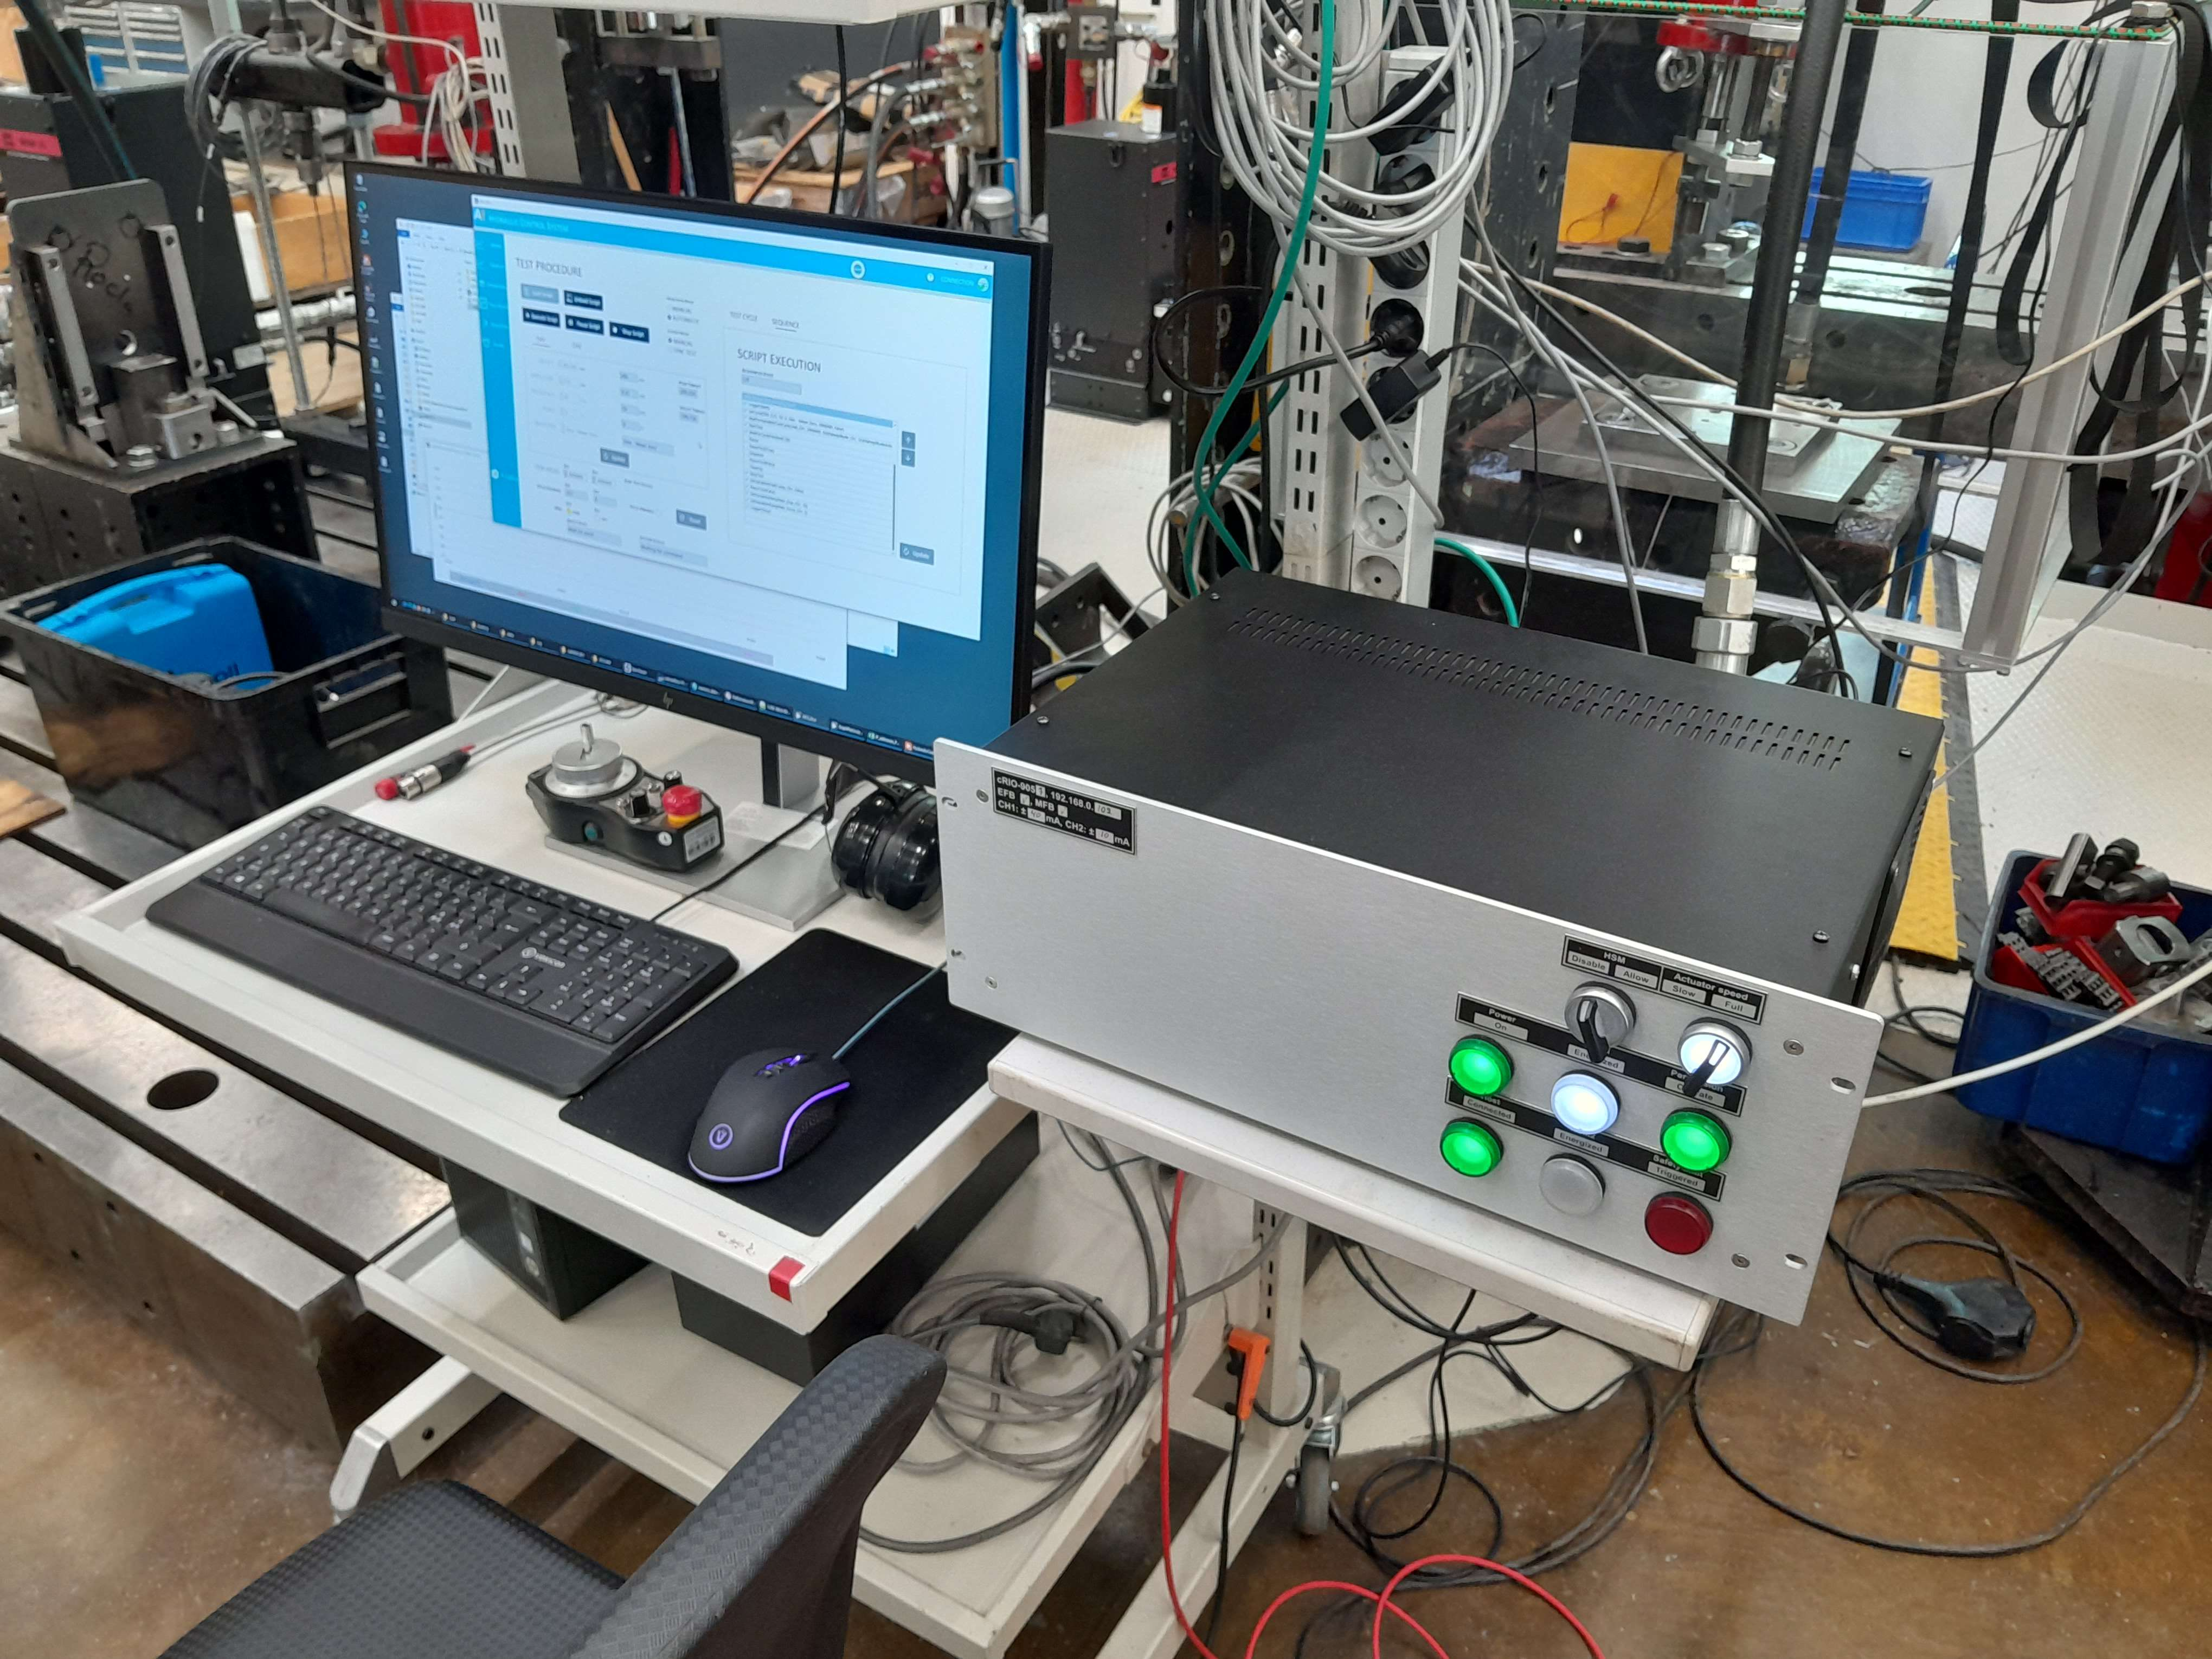
\includegraphics[width=0.98\textwidth]{assets/solid_mechanics_control_monitor}
  \caption{The rack-mountable box on the right contains the analog IO components, the FPGA and CPU, and other supporting electronics.  It's connected to the desktop workstation on the left which can monitor the state of the system, provide an interface for operators to set test schedules, and record data acquisition.  Not pictured is the QuantumX data acquisition and amplifier unit.}\label{fig:solid_mechanics_control_monitor}
\end{figure}

The control layer was built, like the lower layers, with NI tooling.  All of it was built with LabView, with the CPU-based controls using the LabView Real-Time Module~\cite{NIRealTimeModule} and the FPGA controls built with the LabView FPGA Module~\cite{NIFPGAModule}.  It implemented a PID controller, though the derivative term was in practice usually omitted~\cite{Schad2011,Ali2010}.  To monitor the condition of long-running tests and for data acquisition, there are programs running on a desktop workstation, seen in figure~\ref{fig:solid_mechanics_control_monitor}, that observe the state of the control system.  They also developed a custom scripting language that runs on the workstation to define the high-level testing schedule, separate from the low-level control logic.

\begin{figure}[h]
  \centering
  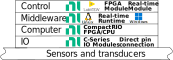
\includegraphics[width=\textwidth]{assets/mechatronic_tech_stack_solid_mechanics}
  \caption{The tech stack is dominated by National Instruments CompactRIO tooling.  Some of the components for the desktop system, like the Windows operating system, are not, but they are the exception.}\label{fig:mechatronic_tech_stack_solid_mechanics}
\end{figure}

The Aalto Solid Mechanics Laboratory's new control system provides a compelling case study on how control components may be selected when there are requirements placed on the control system beyond easy development.  It led to a need for high-speed IO and computation and a computer with multiple computation units with a CPU and an FPGA.\  Its tech stack is illustrated in figure~\ref{fig:mechatronic_tech_stack_solid_mechanics}.  The system as constructed has been able to meet the performance requirements and execute useful tests.  Development is on-going.

\clearpage


\section{Discussion}

This paper has introduced a theory of a mechatronic tech stack which describes function and tooling for mechatronic systems, namely as discrete layers of control, middleware, computer, and IO.\  This theory is motivated by analogy to the web stack, used in IT software development, and to the OSI networking model, used to describe networked computer systems.  The OSI model also provided a means of discriminating the layers that make up the model, importantly by finding contrasts in the morphology, syntax, and semantics of the behavior of components of the control system.

It also tested this theory against several case studies.  In one case, a hydraulic steering linkage test bed showed that a change in one abstraction layer can demand re-architecture of the other abstraction layers if the control system is not carefully designed.  In another, an organization employed variations on one tech stack to build robots based on soft actuators, presumably to capitalize on institutional knowledge of that stack.  Another used the development of a Stewart platform to show how a control system can be developed based on this theory.  The last showed how performance requirements for a strain testing machine can drive the architecture of a control system and how that can be captured by this model.  By organizing the tools used in these case studies based on the function they perform and the interface they provide, I generated compelling insights into the architecture of the control systems.

Although useful, the theory presented is not yet mature.  The largest issue is that the definitions of the abstraction layers and the boundaries between them lack specificity.  For instance, I state that the computer layer is the hardware that performs computation and that the interface it provides is its architecture.  What constitutes such computational hardware, and what exactly is a computer architecture?  And what is a practitioner meant to do with this information?  Stating that a computer uses a SuperH or x86 architecture doesn't immediately suggest which is better for the application, and likewise for a ATmega328P or ATmega32u4 computer chip.  Providing specific definitions for the layers, their boundaries, and how they are parameterized would be useful.

To increase the specificity of the definition of the theory, motivating its definition with more background theory could be appealing.  Presently, it's motivated by an analogy to the web stack and by a test defined in the OSI model.  If even more theories were employed to discern the structure of the stack and they pointed to similar results, that would substantially strengthen the argument for this theory.  A concrete step towards a specific definition for the tech stack theory would be to emulate the layer definitions provided in the OSI model, which enumerate the purpose, provided services, and function of each abstraction layer~\cite[§7]{ISO7498-1}.  However, it would be better to draw from more sources than this one standard for how to structure the definitions in this theory.  Further benefit could be found by studying and creating more case studies to challenge the structure of the theory and to test its utility.

This theory can also be extended.  Throughout this work, it has been called a \textit{mechatronic} tech stack, but truly it's a control system tech stack.  To make it a true mechatronic tech stack, it should include tooling for mechanical and electronic systems.  A mechanical section of the stack would grow from the bottom of the stack shown in figure~\ref{fig:mechatronic_tech_stack}, not colliding with the current stack, but an electrical component would be more complicated, since it is needed by both the mechanical stack for transducers and sensors, and by the control stack since the computer \textit{is} an electrical component, and the IO layer often needs some electrical finesse, as noted in §\ref{sec:stewart_platform}.  It could also be extended in the software realm; the production of graphical monitoring systems and tele-operation programs generally require substantial non-control software which should be described by different layers, perhaps forking away from the middleware layer to have a monitoring layer branch.

This theory would also benefit from the study of adjacent work that doesn't develop the mechatronic tech stack itself.  This theory describes the function of mechatronic tooling, but it provides no notion of what tools are best for a particular application.  In evaluating the case studies, some initial guesses were developed, like that tools should encourage loose coupling, take advantage of institutional knowledge, be easy to troubleshoot, and meet certain performance requirements.  This can be formalized by interviewing practitioners and querying what qualities they value in tools as well as by studying extant literature on the subject of tool quality.  These studies would be synthesized into a coherent model for representing the quality of a tool.  Likely this would manifest as a multi-dimensional model which a practitioner would interpret to get the best result as apposed to a one-dimensional quality rating that gives practitioners no agency.

As well as considering the quality of a tool, it's important also to study the legal existence of mechatronic tools.  Almost always when making and redistributing mechatronic systems and related design assets, engineers and their associated organizations must agree to some license agreement with the authors of their tools, with these legal agreements being underpinned by various intellectual property laws and treaties.  While it is tempting to just ``hit agree'', these license agreements can place notable conditions on their redistribution within mechatronic systems that employ them.  A notable subset of these agreements are those \textit{open-source} licenses, which are often discussed as interesting to practitioners in mechatronics, but the legal requirements for open-source software are often ignored or misunderstood.  Open-hardware licenses are even less understood.  A deep dive into law around mechatronic tools would greatly enhance the mechatronic tech stack theory by allowing practitioners to evaluate if they're even allowed to use a tool, regardless of its quality.

Finally, this theory will not do much benefit locked away in a masters thesis that so few people will ever read.  For it to be truly useful, it must be deployed widely among practitioners of mechatronics.  This can be accomplished in several ways.  The theory and progress on it can be published to journals and conferences (indeed, a subset of this thesis is in review for the Japanese Fluid Power Society's conference~\cite{Porter2024}) or perhaps even to more informal forums like a personal blog or social media.  Collaborating on projects with other research groups and industry and deploying this theory will both spread the ideas of the thesis and test its utility.  Finally, developing teaching for this project would be an useful test of its utility.  Students who don't have much experience with architecting mechatronic systems will have the most useful feedback to whether the structure provided by this theory is truly useful for developing projects.

\clearpage


\section{Conclusion}

This paper presented three case studies to demonstrate the utility of the novel theory of a mechatronic tech stack. These cases were diverse in their applications and methods and by viewing them through the lens of the tech stack, new knowledge of how mechatronic systems can be commissioned was gained. Also, by studying several stacks, I have formed a pool of tools to draw from. The mechatronic tech stack can be re-rendered to reflect this, as here in figure~\ref{fig:mechatronic_tech_stack_filled}.

\begin{figure}[h]
  \centering
  \includegraphics[width=\textwidth]{assets/mechatronic_tech_stack_filled}
  \caption{The mechatronic tech stack for all of the case studies in one, with tools for each project highlighted in different colors.  Not only does the mechatronic tech stack present layers of abstraction, it also provides an idea of what tools to choose, similar to the web stack in figure~\ref{fig:web_stack}.}\label{fig:mechatronic_tech_stack_filled}
\end{figure}

This model can be improved by conducting more retrospective analyses, like those done for Dolores and the EFPA projects, to better model existing systems. Further, executing more projects using this theory will test and exercise its utility. The scope of the model can also be increased; instead of only modeling control systems, it could be expanded to model mechanical, electrical, or fluid systems.

This thesis has also set forth a trajectory for future work in this topic, including expanding the scope of the tech stack from only control components to also hardware components, modeling the quality of tooling, and studying related topics like open-source software.  All this will be done in the author's doctoral studies.

Using this model, practitioners can more easily reason about what different parts of their control systems do and what tools to employ for them. This mental model enables faster development of systems and redirects thought to what tools would be best instead of merely functional. All this will allay the difficulty and complexity of developing fluid power systems.

\clearpage

\phantomsection
\addcontentsline{toc}{section}{\refname}
%%\addcontentsline{toc}{section}{References}

\bibliographystyle{ieeetr}
\bibliography{bib/good-masters.bib}

\end{document}
